% Options for packages loaded elsewhere
\PassOptionsToPackage{unicode}{hyperref}
\PassOptionsToPackage{hyphens}{url}
%
\documentclass[
]{article}
\usepackage{amsmath,amssymb}
\usepackage{lmodern}
\usepackage{iftex}
\ifPDFTeX
  \usepackage[T1]{fontenc}
  \usepackage[utf8]{inputenc}
  \usepackage{textcomp} % provide euro and other symbols
\else % if luatex or xetex
  \usepackage{unicode-math}
  \defaultfontfeatures{Scale=MatchLowercase}
  \defaultfontfeatures[\rmfamily]{Ligatures=TeX,Scale=1}
\fi
% Use upquote if available, for straight quotes in verbatim environments
\IfFileExists{upquote.sty}{\usepackage{upquote}}{}
\IfFileExists{microtype.sty}{% use microtype if available
  \usepackage[]{microtype}
  \UseMicrotypeSet[protrusion]{basicmath} % disable protrusion for tt fonts
}{}
\makeatletter
\@ifundefined{KOMAClassName}{% if non-KOMA class
  \IfFileExists{parskip.sty}{%
    \usepackage{parskip}
  }{% else
    \setlength{\parindent}{0pt}
    \setlength{\parskip}{6pt plus 2pt minus 1pt}}
}{% if KOMA class
  \KOMAoptions{parskip=half}}
\makeatother
\usepackage{xcolor}
\usepackage[margin=1in]{geometry}
\usepackage{color}
\usepackage{fancyvrb}
\newcommand{\VerbBar}{|}
\newcommand{\VERB}{\Verb[commandchars=\\\{\}]}
\DefineVerbatimEnvironment{Highlighting}{Verbatim}{commandchars=\\\{\}}
% Add ',fontsize=\small' for more characters per line
\usepackage{framed}
\definecolor{shadecolor}{RGB}{248,248,248}
\newenvironment{Shaded}{\begin{snugshade}}{\end{snugshade}}
\newcommand{\AlertTok}[1]{\textcolor[rgb]{0.94,0.16,0.16}{#1}}
\newcommand{\AnnotationTok}[1]{\textcolor[rgb]{0.56,0.35,0.01}{\textbf{\textit{#1}}}}
\newcommand{\AttributeTok}[1]{\textcolor[rgb]{0.77,0.63,0.00}{#1}}
\newcommand{\BaseNTok}[1]{\textcolor[rgb]{0.00,0.00,0.81}{#1}}
\newcommand{\BuiltInTok}[1]{#1}
\newcommand{\CharTok}[1]{\textcolor[rgb]{0.31,0.60,0.02}{#1}}
\newcommand{\CommentTok}[1]{\textcolor[rgb]{0.56,0.35,0.01}{\textit{#1}}}
\newcommand{\CommentVarTok}[1]{\textcolor[rgb]{0.56,0.35,0.01}{\textbf{\textit{#1}}}}
\newcommand{\ConstantTok}[1]{\textcolor[rgb]{0.00,0.00,0.00}{#1}}
\newcommand{\ControlFlowTok}[1]{\textcolor[rgb]{0.13,0.29,0.53}{\textbf{#1}}}
\newcommand{\DataTypeTok}[1]{\textcolor[rgb]{0.13,0.29,0.53}{#1}}
\newcommand{\DecValTok}[1]{\textcolor[rgb]{0.00,0.00,0.81}{#1}}
\newcommand{\DocumentationTok}[1]{\textcolor[rgb]{0.56,0.35,0.01}{\textbf{\textit{#1}}}}
\newcommand{\ErrorTok}[1]{\textcolor[rgb]{0.64,0.00,0.00}{\textbf{#1}}}
\newcommand{\ExtensionTok}[1]{#1}
\newcommand{\FloatTok}[1]{\textcolor[rgb]{0.00,0.00,0.81}{#1}}
\newcommand{\FunctionTok}[1]{\textcolor[rgb]{0.00,0.00,0.00}{#1}}
\newcommand{\ImportTok}[1]{#1}
\newcommand{\InformationTok}[1]{\textcolor[rgb]{0.56,0.35,0.01}{\textbf{\textit{#1}}}}
\newcommand{\KeywordTok}[1]{\textcolor[rgb]{0.13,0.29,0.53}{\textbf{#1}}}
\newcommand{\NormalTok}[1]{#1}
\newcommand{\OperatorTok}[1]{\textcolor[rgb]{0.81,0.36,0.00}{\textbf{#1}}}
\newcommand{\OtherTok}[1]{\textcolor[rgb]{0.56,0.35,0.01}{#1}}
\newcommand{\PreprocessorTok}[1]{\textcolor[rgb]{0.56,0.35,0.01}{\textit{#1}}}
\newcommand{\RegionMarkerTok}[1]{#1}
\newcommand{\SpecialCharTok}[1]{\textcolor[rgb]{0.00,0.00,0.00}{#1}}
\newcommand{\SpecialStringTok}[1]{\textcolor[rgb]{0.31,0.60,0.02}{#1}}
\newcommand{\StringTok}[1]{\textcolor[rgb]{0.31,0.60,0.02}{#1}}
\newcommand{\VariableTok}[1]{\textcolor[rgb]{0.00,0.00,0.00}{#1}}
\newcommand{\VerbatimStringTok}[1]{\textcolor[rgb]{0.31,0.60,0.02}{#1}}
\newcommand{\WarningTok}[1]{\textcolor[rgb]{0.56,0.35,0.01}{\textbf{\textit{#1}}}}
\usepackage{graphicx}
\makeatletter
\def\maxwidth{\ifdim\Gin@nat@width>\linewidth\linewidth\else\Gin@nat@width\fi}
\def\maxheight{\ifdim\Gin@nat@height>\textheight\textheight\else\Gin@nat@height\fi}
\makeatother
% Scale images if necessary, so that they will not overflow the page
% margins by default, and it is still possible to overwrite the defaults
% using explicit options in \includegraphics[width, height, ...]{}
\setkeys{Gin}{width=\maxwidth,height=\maxheight,keepaspectratio}
% Set default figure placement to htbp
\makeatletter
\def\fps@figure{htbp}
\makeatother
\setlength{\emergencystretch}{3em} % prevent overfull lines
\providecommand{\tightlist}{%
  \setlength{\itemsep}{0pt}\setlength{\parskip}{0pt}}
\setcounter{secnumdepth}{5}
\ifLuaTeX
  \usepackage{selnolig}  % disable illegal ligatures
\fi
\IfFileExists{bookmark.sty}{\usepackage{bookmark}}{\usepackage{hyperref}}
\IfFileExists{xurl.sty}{\usepackage{xurl}}{} % add URL line breaks if available
\urlstyle{same} % disable monospaced font for URLs
\hypersetup{
  pdftitle={Taller 2 Regresión lineal Multiple},
  pdfauthor={Andrés Felipe Palomino - David Stiven Rojas},
  hidelinks,
  pdfcreator={LaTeX via pandoc}}

\title{Taller 2 Regresión lineal Multiple}
\author{Andrés Felipe Palomino - David Stiven Rojas}
\date{2023-04-21}

\begin{document}
\maketitle

\hypertarget{introducciuxf3n}{%
\section{Introducción}\label{introducciuxf3n}}

La base de datos \("yarn"\) obtenida de la librería (PLS) contiene
información sobre espectros NIR y mediciones de densidad de hilos de
PET, consta de 28 individuos (hilos de PET), 268 variables predictoras
(NIRS) y una variable de respuesta (densidad). Se ajustará un modelo
lineal múltiple para estimar la densidad del hilo PET, mediante
mediciones NIR

\begin{Shaded}
\begin{Highlighting}[]
\CommentTok{\#Importación de librerías necesarias}
\NormalTok{lib\_req}\OtherTok{\textless{}{-}}\FunctionTok{c}\NormalTok{(}\StringTok{"glmnet"}\NormalTok{,}\StringTok{"lmridge"}\NormalTok{,}\StringTok{"scatterplot3d"}\NormalTok{,}\StringTok{"plot3D"}\NormalTok{,}\StringTok{"plotly"}\NormalTok{,}\StringTok{"rgl"}\NormalTok{,}\StringTok{"plot3Drgl"}\NormalTok{,}
           \StringTok{\textquotesingle{}effects\textquotesingle{}}\NormalTok{,}\StringTok{\textquotesingle{}psych\textquotesingle{}}\NormalTok{,}
           \StringTok{\textquotesingle{}car\textquotesingle{}}\NormalTok{,}\StringTok{\textquotesingle{}lmtest\textquotesingle{}}\NormalTok{,}\StringTok{\textquotesingle{}MASS\textquotesingle{}}\NormalTok{,}\StringTok{\textquotesingle{}latex2exp\textquotesingle{}}\NormalTok{,}\StringTok{\textquotesingle{}orcutt\textquotesingle{}}\NormalTok{,}
           \StringTok{\textquotesingle{}nlme\textquotesingle{}}\NormalTok{,}\StringTok{"zoom"}\NormalTok{,}\StringTok{\textquotesingle{}ggfortify\textquotesingle{}}\NormalTok{,}\StringTok{\textquotesingle{}readxl\textquotesingle{}}\NormalTok{,}\StringTok{\textquotesingle{}pls\textquotesingle{}}\NormalTok{)}\CommentTok{\# Listado de librerias requeridas por el script}
\NormalTok{easypackages}\SpecialCharTok{::}\FunctionTok{packages}\NormalTok{(lib\_req)}
\end{Highlighting}
\end{Shaded}

\hypertarget{base-de-datos}{%
\subsection{Base de datos}\label{base-de-datos}}

En la siguiente tabla se encuentra un encabezado de la base de datos que
se trabajara, esta consta de 30 covariables predictoras, las cuales
estarán desde NIR1 hasta NIR30. De primera mano se observa que los
valores de los NIR disminuyen a medida que la covariable aumenta

\begin{Shaded}
\begin{Highlighting}[]
\NormalTok{X }\OtherTok{\textless{}{-}} \FunctionTok{data.frame}\NormalTok{(}\FunctionTok{matrix}\NormalTok{(}\FunctionTok{c}\NormalTok{(yarn}\SpecialCharTok{$}\NormalTok{NIR[,}\DecValTok{1}\SpecialCharTok{:}\DecValTok{30}\NormalTok{],yarn}\SpecialCharTok{$}\NormalTok{density),}\AttributeTok{nrow =}\DecValTok{28}\NormalTok{, }\AttributeTok{ncol=} \DecValTok{31}\NormalTok{))}
\FunctionTok{colnames}\NormalTok{(X) }\OtherTok{\textless{}{-}} \FunctionTok{c}\NormalTok{(}\FunctionTok{paste}\NormalTok{(}\StringTok{"NIR"}\NormalTok{,}\DecValTok{1}\SpecialCharTok{:}\DecValTok{30}\NormalTok{,}\AttributeTok{sep=}\StringTok{""}\NormalTok{),}\StringTok{"density"}\NormalTok{)}
\end{Highlighting}
\end{Shaded}

\hypertarget{funciones-creadas}{%
\subsection{Funciones creadas}\label{funciones-creadas}}

Antes de empezar con el proceso de seleccionar las variables para
ajustar el modelo se crean funciones para optimizar el proceso de
validación de supuestos, debido a que constantemente se deben realizar,
estas funciones estan diseñadas para objetos lm.

\begin{Shaded}
\begin{Highlighting}[]
\DocumentationTok{\#\#Validacion grafica para homocedasticidad y normalidad y pruebas formales}
\NormalTok{validaciongrafica}\OtherTok{\textless{}{-}} \ControlFlowTok{function}\NormalTok{(model,}\AttributeTok{cor=}\NormalTok{F)\{}
  
  \FunctionTok{par}\NormalTok{(}\AttributeTok{mfrow=}\FunctionTok{c}\NormalTok{(}\DecValTok{1}\NormalTok{,}\DecValTok{2}\NormalTok{))}
  \FunctionTok{plot}\NormalTok{(}\FunctionTok{fitted.values}\NormalTok{(model),}\FunctionTok{studres}\NormalTok{(model),}\AttributeTok{panel.first=}\FunctionTok{grid}\NormalTok{(),}
       \AttributeTok{pch=}\DecValTok{19}\NormalTok{,}\AttributeTok{ylab=}\StringTok{\textquotesingle{}Residuos Estudentizados\textquotesingle{}}\NormalTok{,}\AttributeTok{xlab=}\StringTok{\textquotesingle{}Valores ajustados\textquotesingle{}}\NormalTok{,}\AttributeTok{main=}\StringTok{\textquotesingle{}A\textquotesingle{}}\NormalTok{,}\AttributeTok{col=}\StringTok{\textquotesingle{}aquamarine4\textquotesingle{}}\NormalTok{)}
  \FunctionTok{abline}\NormalTok{(}\AttributeTok{h=}\FunctionTok{c}\NormalTok{(}\SpecialCharTok{{-}}\DecValTok{2}\NormalTok{,}\DecValTok{0}\NormalTok{,}\DecValTok{2}\NormalTok{),}\AttributeTok{lty=}\DecValTok{2}\NormalTok{)}
  \FunctionTok{qqPlot}\NormalTok{(model,}\AttributeTok{pch=}\DecValTok{19}\NormalTok{,}\AttributeTok{ylab=}\StringTok{\textquotesingle{}Residuos Estudentizados\textquotesingle{}}\NormalTok{,}
         \AttributeTok{xlab=}\StringTok{\textquotesingle{}Cuantiles Teóricos\textquotesingle{}}\NormalTok{,}\AttributeTok{col=}\FunctionTok{carPalette}\NormalTok{()[}\DecValTok{1}\NormalTok{],}
         \AttributeTok{col.lines=}\FunctionTok{carPalette}\NormalTok{()[}\DecValTok{3}\NormalTok{],}\AttributeTok{main=}\StringTok{\textquotesingle{}B\textquotesingle{}}\NormalTok{)}
  \FunctionTok{print}\NormalTok{(}\StringTok{\textquotesingle{}Shapiro Test; H0: Normalidad vs H1: No Normalidad\textquotesingle{}}\NormalTok{)}
  \FunctionTok{print}\NormalTok{(}\FunctionTok{shapiro.test}\NormalTok{(}\FunctionTok{studres}\NormalTok{(model)))}
  \FunctionTok{print}\NormalTok{(}\StringTok{\textquotesingle{}Breusch Pagan Test;H0: Homocedasticidad vs H1: No Homocedasticidad\textquotesingle{}}\NormalTok{)}
  \FunctionTok{print}\NormalTok{(}\FunctionTok{bptest}\NormalTok{(model))}
  \ControlFlowTok{if}\NormalTok{(cor}\SpecialCharTok{==}\NormalTok{T)\{}
    \FunctionTok{par}\NormalTok{(}\AttributeTok{mfrow=}\FunctionTok{c}\NormalTok{(}\DecValTok{1}\NormalTok{,}\DecValTok{2}\NormalTok{))}
    \FunctionTok{plot}\NormalTok{(}\FunctionTok{studres}\NormalTok{(model),}\AttributeTok{type=}\StringTok{"b"}\NormalTok{,}\AttributeTok{xlab=}\StringTok{"Tiempo"}\NormalTok{,}\AttributeTok{ylab=}\StringTok{"Residuos Estudentizados"}\NormalTok{,}\AttributeTok{main=}\StringTok{"A"}\NormalTok{,}
         \AttributeTok{pch=}\DecValTok{19}\NormalTok{,}\AttributeTok{panel.first=}\FunctionTok{grid}\NormalTok{())}
    \FunctionTok{plot}\NormalTok{(}\FunctionTok{studres}\NormalTok{(model)[}\SpecialCharTok{{-}}\FunctionTok{length}\NormalTok{(}\FunctionTok{fitted.values}\NormalTok{(model))],}
         \FunctionTok{studres}\NormalTok{(model)[}\SpecialCharTok{{-}}\DecValTok{1}\NormalTok{],}\AttributeTok{pch=}\DecValTok{19}\NormalTok{,}\AttributeTok{panel.first =} \FunctionTok{grid}\NormalTok{(),}\AttributeTok{col=}\StringTok{"turquoise3"}\NormalTok{,}
         \AttributeTok{xlab=}\FunctionTok{TeX}\NormalTok{(}\StringTok{"$Residuos\_\{t{-}1\}$"}\NormalTok{),}\AttributeTok{ylab=}\FunctionTok{TeX}\NormalTok{(}\StringTok{"$Residuos\_\{t\}$"}\NormalTok{),}\AttributeTok{main=}\StringTok{"B"}\NormalTok{)}
    \FunctionTok{abline}\NormalTok{(}\FunctionTok{lm}\NormalTok{(}\FunctionTok{studres}\NormalTok{(model)[}\SpecialCharTok{{-}}\DecValTok{1}\NormalTok{]}\SpecialCharTok{\textasciitilde{}}\FunctionTok{studres}\NormalTok{(model)[}\SpecialCharTok{{-}}\FunctionTok{length}\NormalTok{(}\FunctionTok{fitted.values}\NormalTok{(model))]))}
    \FunctionTok{print}\NormalTok{(}\StringTok{\textquotesingle{}Durbin Watson Test\textquotesingle{}}\NormalTok{)}
    \FunctionTok{print}\NormalTok{(}\FunctionTok{durbinWatsonTest}\NormalTok{(model,}
                           \AttributeTok{method=}\StringTok{\textquotesingle{}resample\textquotesingle{}}\NormalTok{,}\AttributeTok{reps=}\DecValTok{10000}\NormalTok{))}
\NormalTok{  \}}
  \FunctionTok{par}\NormalTok{(}\AttributeTok{mfrow=}\FunctionTok{c}\NormalTok{(}\DecValTok{1}\NormalTok{,}\DecValTok{1}\NormalTok{))}
\NormalTok{\}}

\DocumentationTok{\#\# Calculo de lambda optimo para boxcox}
\NormalTok{lambda}\OtherTok{\textless{}{-}} \ControlFlowTok{function}\NormalTok{(model,a,b)\{}
  \FunctionTok{par}\NormalTok{(}\AttributeTok{mfrow=}\FunctionTok{c}\NormalTok{(}\DecValTok{1}\NormalTok{,}\DecValTok{1}\NormalTok{))}
\NormalTok{  box.cox}\OtherTok{\textless{}{-}}\FunctionTok{boxcox}\NormalTok{(model,}\AttributeTok{lambda=}\FunctionTok{seq}\NormalTok{(a,b,}\AttributeTok{length.out =} \DecValTok{1000}\NormalTok{),}
                  \AttributeTok{ylab=}\StringTok{\textquotesingle{}log{-}verosimilitud\textquotesingle{}}\NormalTok{)}
\NormalTok{  bc}\OtherTok{\textless{}{-}}\FunctionTok{round}\NormalTok{(box.cox}\SpecialCharTok{$}\NormalTok{x[box.cox}\SpecialCharTok{$}\NormalTok{y }\SpecialCharTok{==}\FunctionTok{max}\NormalTok{(box.cox}\SpecialCharTok{$}\NormalTok{y)],}\DecValTok{2}\NormalTok{)}
  \FunctionTok{print}\NormalTok{(bc)}
\NormalTok{\}}
\end{Highlighting}
\end{Shaded}

Antes de generar el proceso de selección de variables recordaremos
brevemente que una regresión lineal múltiple no es el conjunto de la
suma de regresiones lineales simples, es decir estamos trabajando con
espacios generados en función de un conjunto de covariables. Por lo cuál
haremos un breve ejercicio ilustrativo de como se evidencia esto. En el
diagrama de dispersión inicial vemos que la relación entre las
covariables no se evidenciaba de una manera fuerte lineal, con
coeficientes de correlación lineal débiles, pero en el diagrama de
dispersión en 3D se nota relaciones fuertes.

\begin{Shaded}
\begin{Highlighting}[]
\FunctionTok{par}\NormalTok{(}\AttributeTok{mfrow=}\FunctionTok{c}\NormalTok{(}\DecValTok{1}\NormalTok{,}\DecValTok{2}\NormalTok{))}
\NormalTok{psych}\SpecialCharTok{::}\FunctionTok{pairs.panels}\NormalTok{(X[,}\FunctionTok{c}\NormalTok{(}\DecValTok{31}\NormalTok{,}\DecValTok{4}\NormalTok{,}\DecValTok{29}\NormalTok{)], }
                      \AttributeTok{method =} \StringTok{"pearson"}\NormalTok{, }\CommentTok{\# correlation method}
                      \AttributeTok{hist.col =} \StringTok{"aquamarine1"}\NormalTok{,}
                      \AttributeTok{density =} \ConstantTok{TRUE}\NormalTok{,  }\CommentTok{\# show density plots}
                      \AttributeTok{ellipses =} \ConstantTok{TRUE} \CommentTok{\# show correlation ellipses}
\NormalTok{  )}
\end{Highlighting}
\end{Shaded}

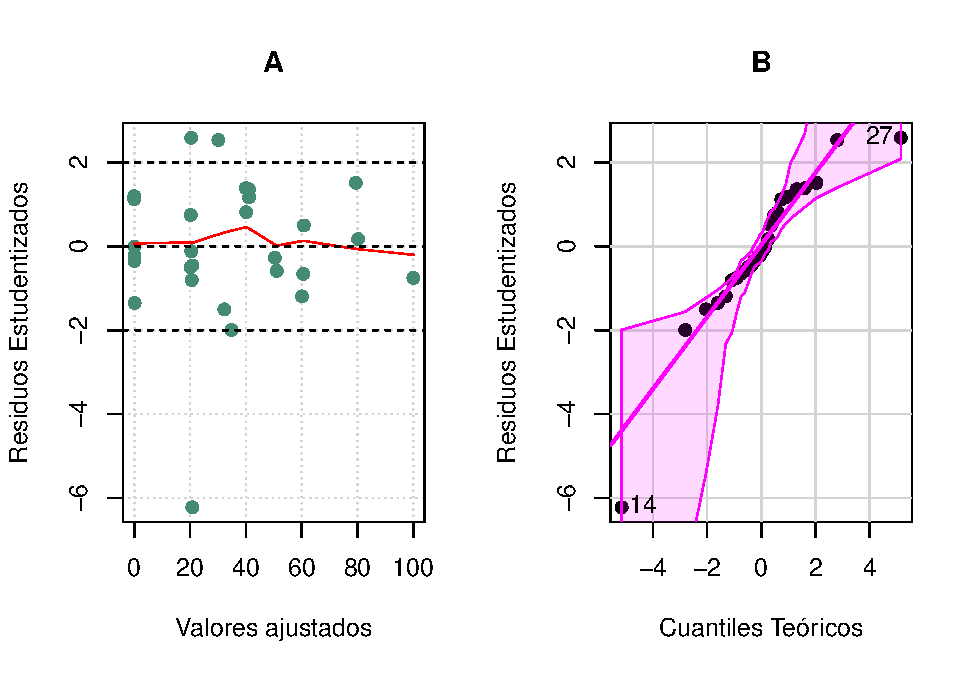
\includegraphics{Taller-2-Regresion-Multiple-Aplicada_files/figure-latex/unnamed-chunk-4-1.pdf}

\begin{Shaded}
\begin{Highlighting}[]
\NormalTok{z}\OtherTok{\textless{}{-}}\NormalTok{X[,}\DecValTok{31}\NormalTok{];y}\OtherTok{\textless{}{-}}\NormalTok{X[,}\DecValTok{4}\NormalTok{];x}\OtherTok{\textless{}{-}}\NormalTok{X[,}\DecValTok{29}\NormalTok{];}
\FunctionTok{scatter3D}\NormalTok{(x, y, z, }\AttributeTok{phi =} \DecValTok{0}\NormalTok{, }\AttributeTok{bty =} \StringTok{"b2"}\NormalTok{,}\AttributeTok{col =} \FunctionTok{c}\NormalTok{(}\StringTok{\textquotesingle{}aquamarine\textquotesingle{}}\NormalTok{,}\StringTok{\textquotesingle{}aquamarine2\textquotesingle{}}\NormalTok{,}\StringTok{\textquotesingle{}aquamarine3\textquotesingle{}}\NormalTok{,}\StringTok{\textquotesingle{}dodgerblue\textquotesingle{}}\NormalTok{,}
\StringTok{\textquotesingle{}dodgerblue2\textquotesingle{}}\NormalTok{,}\StringTok{\textquotesingle{}dodgerblue3\textquotesingle{}}\NormalTok{,}\StringTok{\textquotesingle{}dodgerblue4\textquotesingle{}}\NormalTok{),}\AttributeTok{pch =} \DecValTok{20}\NormalTok{, }\AttributeTok{cex =} \DecValTok{2}\NormalTok{, }
\AttributeTok{ticktype =} \StringTok{"detailed"}\NormalTok{,}\AttributeTok{xlab=}\StringTok{\textquotesingle{}NIR29\textquotesingle{}}\NormalTok{,}\AttributeTok{ylab=}\StringTok{\textquotesingle{}NIR 4\textquotesingle{}}\NormalTok{, }\AttributeTok{zlab=}\StringTok{\textquotesingle{}Density\textquotesingle{}}\NormalTok{)}
\CommentTok{\#Creamos un objeto para realizar las predicciones con elmodelo}
\NormalTok{objr}\OtherTok{\textless{}{-}}\FunctionTok{lm}\NormalTok{(z }\SpecialCharTok{\textasciitilde{}}\NormalTok{ x}\SpecialCharTok{+}\NormalTok{y)}
\FunctionTok{summary}\NormalTok{(objr)}
\end{Highlighting}
\end{Shaded}

\begin{verbatim}
## 
## Call:
## lm(formula = z ~ x + y)
## 
## Residuals:
##     Min      1Q  Median      3Q     Max 
## -7.3050 -4.8871 -0.7899  2.2812 10.7069 
## 
## Coefficients:
##             Estimate Std. Error t value Pr(>|t|)    
## (Intercept)  -24.845     17.179  -1.446    0.161    
## x           -180.297      8.987 -20.063  < 2e-16 ***
## y             97.698      5.459  17.896 9.15e-16 ***
## ---
## Signif. codes:  0 '***' 0.001 '**' 0.01 '*' 0.05 '.' 0.1 ' ' 1
## 
## Residual standard error: 5.66 on 25 degrees of freedom
## Multiple R-squared:  0.9592, Adjusted R-squared:  0.9559 
## F-statistic: 293.9 on 2 and 25 DF,  p-value: < 2.2e-16
\end{verbatim}

\begin{Shaded}
\begin{Highlighting}[]
\CommentTok{\#preparamos el modelado 3d}
\NormalTok{grid.lines }\OtherTok{=} \DecValTok{42}
\NormalTok{x.pred }\OtherTok{\textless{}{-}} \FunctionTok{seq}\NormalTok{(}\FunctionTok{min}\NormalTok{(x), }\FunctionTok{max}\NormalTok{(x), }\AttributeTok{length.out =}\NormalTok{ grid.lines)}


\NormalTok{y.pred }\OtherTok{\textless{}{-}} \FunctionTok{seq}\NormalTok{(}\FunctionTok{min}\NormalTok{(y), }\FunctionTok{max}\NormalTok{(y), }\AttributeTok{length.out =}\NormalTok{ grid.lines)}
\NormalTok{xy }\OtherTok{\textless{}{-}} \FunctionTok{expand.grid}\NormalTok{( }\AttributeTok{x =}\NormalTok{ x.pred, }\AttributeTok{y =}\NormalTok{ y.pred)}
\NormalTok{z.pred }\OtherTok{\textless{}{-}} \FunctionTok{matrix}\NormalTok{(}\FunctionTok{predict}\NormalTok{(objr, }\AttributeTok{newdata =}\NormalTok{ xy), }
                 \AttributeTok{nrow =}\NormalTok{ grid.lines, }\AttributeTok{ncol =}\NormalTok{ grid.lines)}
\CommentTok{\# Marcamos las líneas de iteracción para que busquen la recta de regresión}
\NormalTok{fitpoints }\OtherTok{\textless{}{-}} \FunctionTok{predict}\NormalTok{(objr)}
\CommentTok{\#ploteamos la gráfica en 3d con recta de regresión}
\FunctionTok{scatter3D}\NormalTok{(x, y, z, }\AttributeTok{pch =} \DecValTok{19}\NormalTok{, }\AttributeTok{cex =} \DecValTok{2}\NormalTok{, }
\AttributeTok{theta =} \DecValTok{20}\NormalTok{, }\AttributeTok{phi =} \DecValTok{20}\NormalTok{, }\AttributeTok{ticktype =} \StringTok{"detailed"}\NormalTok{,}
\AttributeTok{surf =} \FunctionTok{list}\NormalTok{(}\AttributeTok{x =}\NormalTok{ x.pred, }\AttributeTok{y =}\NormalTok{ y.pred, }\AttributeTok{z =}\NormalTok{ z.pred,}\AttributeTok{facets =} \ConstantTok{NA}\NormalTok{, }\AttributeTok{fit =}\NormalTok{ fitpoints), }
\AttributeTok{main =} \StringTok{""}\NormalTok{,}\AttributeTok{xlab=}\StringTok{\textquotesingle{}NIR29 \textquotesingle{}}\NormalTok{,}\AttributeTok{zlab=}\StringTok{"Density"}\NormalTok{,}\AttributeTok{ylab=}\StringTok{\textquotesingle{}NIR4\textquotesingle{}}\NormalTok{, }
\AttributeTok{col =} \FunctionTok{c}\NormalTok{(}\StringTok{\textquotesingle{}aquamarine\textquotesingle{}}\NormalTok{,}\StringTok{\textquotesingle{}aquamarine2\textquotesingle{}}\NormalTok{,}\StringTok{\textquotesingle{}aquamarine3\textquotesingle{}}\NormalTok{,}
\StringTok{\textquotesingle{}dodgerblue\textquotesingle{}}\NormalTok{,}\StringTok{\textquotesingle{}dodgerblue2\textquotesingle{}}\NormalTok{,}\StringTok{\textquotesingle{}dodgerblue3\textquotesingle{}}\NormalTok{,}\StringTok{\textquotesingle{}dodgerblue4\textquotesingle{}}\NormalTok{))}
\end{Highlighting}
\end{Shaded}

\includegraphics{Taller-2-Regresion-Multiple-Aplicada_files/figure-latex/unnamed-chunk-4-2.pdf}

\begin{Shaded}
\begin{Highlighting}[]
\FunctionTok{par}\NormalTok{(}\AttributeTok{mfrow=}\FunctionTok{c}\NormalTok{(}\DecValTok{1}\NormalTok{,}\DecValTok{2}\NormalTok{))}
\NormalTok{psych}\SpecialCharTok{::}\FunctionTok{pairs.panels}\NormalTok{(X[,}\FunctionTok{c}\NormalTok{(}\DecValTok{31}\NormalTok{,}\DecValTok{2}\NormalTok{,}\DecValTok{18}\NormalTok{)], }
                      \AttributeTok{method =} \StringTok{"pearson"}\NormalTok{, }\CommentTok{\# correlation method}
                      \AttributeTok{hist.col =} \StringTok{"aquamarine1"}\NormalTok{,}
                      \AttributeTok{density =} \ConstantTok{TRUE}\NormalTok{,  }\CommentTok{\# show density plots}
                      \AttributeTok{ellipses =} \ConstantTok{TRUE} \CommentTok{\# show correlation ellipses}
\NormalTok{  )}
\end{Highlighting}
\end{Shaded}

\includegraphics{Taller-2-Regresion-Multiple-Aplicada_files/figure-latex/unnamed-chunk-4-3.pdf}

\begin{Shaded}
\begin{Highlighting}[]
\NormalTok{z}\OtherTok{\textless{}{-}}\NormalTok{X[,}\DecValTok{31}\NormalTok{];y}\OtherTok{\textless{}{-}}\NormalTok{X[,}\DecValTok{2}\NormalTok{];x}\OtherTok{\textless{}{-}}\NormalTok{X[,}\DecValTok{18}\NormalTok{];}
\FunctionTok{scatter3D}\NormalTok{(x, y, z, }\AttributeTok{phi =} \DecValTok{0}\NormalTok{, }\AttributeTok{bty =} \StringTok{"b2"}\NormalTok{,}\AttributeTok{col =} \FunctionTok{c}\NormalTok{(}\StringTok{\textquotesingle{}aquamarine\textquotesingle{}}\NormalTok{,}\StringTok{\textquotesingle{}aquamarine2\textquotesingle{}}\NormalTok{,}\StringTok{\textquotesingle{}aquamarine3\textquotesingle{}}\NormalTok{,}\StringTok{\textquotesingle{}dodgerblue\textquotesingle{}}\NormalTok{,}
\StringTok{\textquotesingle{}dodgerblue2\textquotesingle{}}\NormalTok{,}\StringTok{\textquotesingle{}dodgerblue3\textquotesingle{}}\NormalTok{,}\StringTok{\textquotesingle{}dodgerblue4\textquotesingle{}}\NormalTok{),}\AttributeTok{pch =} \DecValTok{20}\NormalTok{, }\AttributeTok{cex =} \DecValTok{2}\NormalTok{,}
\AttributeTok{ticktype =} \StringTok{"detailed"}\NormalTok{,}
\AttributeTok{xlab=}\StringTok{\textquotesingle{}NIR18\textquotesingle{}}\NormalTok{,}\AttributeTok{ylab=}\StringTok{\textquotesingle{}NIR 2\textquotesingle{}}\NormalTok{, }\AttributeTok{zlab=}\StringTok{\textquotesingle{}Density\textquotesingle{}}\NormalTok{)}
\CommentTok{\#Creamos un objeto para realizar las predicciones con elmodelo}
\NormalTok{objr}\OtherTok{\textless{}{-}}\FunctionTok{lm}\NormalTok{(z }\SpecialCharTok{\textasciitilde{}}\NormalTok{ x}\SpecialCharTok{+}\NormalTok{y)}
\FunctionTok{summary}\NormalTok{(objr)}
\end{Highlighting}
\end{Shaded}

\begin{verbatim}
## 
## Call:
## lm(formula = z ~ x + y)
## 
## Residuals:
##     Min      1Q  Median      3Q     Max 
## -21.003 -10.014  -3.323   9.239  32.444 
## 
## Coefficients:
##             Estimate Std. Error t value Pr(>|t|)    
## (Intercept) -443.361     96.022  -4.617    1e-04 ***
## x            -30.451      4.865  -6.259 1.51e-06 ***
## y            176.813     32.168   5.497 1.04e-05 ***
## ---
## Signif. codes:  0 '***' 0.001 '**' 0.01 '*' 0.05 '.' 0.1 ' ' 1
## 
## Residual standard error: 15.84 on 25 degrees of freedom
## Multiple R-squared:  0.6805, Adjusted R-squared:  0.655 
## F-statistic: 26.63 on 2 and 25 DF,  p-value: 6.389e-07
\end{verbatim}

\begin{Shaded}
\begin{Highlighting}[]
\CommentTok{\#preparamos el modelado 3d}
\NormalTok{grid.lines }\OtherTok{=} \DecValTok{42}
\NormalTok{x.pred }\OtherTok{\textless{}{-}} \FunctionTok{seq}\NormalTok{(}\FunctionTok{min}\NormalTok{(x), }\FunctionTok{max}\NormalTok{(x), }\AttributeTok{length.out =}\NormalTok{ grid.lines)}


\NormalTok{y.pred }\OtherTok{\textless{}{-}} \FunctionTok{seq}\NormalTok{(}\FunctionTok{min}\NormalTok{(y), }\FunctionTok{max}\NormalTok{(y), }\AttributeTok{length.out =}\NormalTok{ grid.lines)}
\NormalTok{xy }\OtherTok{\textless{}{-}} \FunctionTok{expand.grid}\NormalTok{( }\AttributeTok{x =}\NormalTok{ x.pred, }\AttributeTok{y =}\NormalTok{ y.pred)}
\NormalTok{z.pred }\OtherTok{\textless{}{-}} \FunctionTok{matrix}\NormalTok{(}\FunctionTok{predict}\NormalTok{(objr, }\AttributeTok{newdata =}\NormalTok{ xy), }
                 \AttributeTok{nrow =}\NormalTok{ grid.lines, }\AttributeTok{ncol =}\NormalTok{ grid.lines)}
\CommentTok{\# Marcamos las líneas de iteracción para que busquen la recta de regresión}
\NormalTok{fitpoints }\OtherTok{\textless{}{-}} \FunctionTok{predict}\NormalTok{(objr)}
\CommentTok{\#ploteamos la gráfica en 3d con recta de regresión}
\FunctionTok{scatter3D}\NormalTok{(x, y, z, }\AttributeTok{pch =} \DecValTok{19}\NormalTok{, }\AttributeTok{cex =} \DecValTok{2}\NormalTok{, }
\AttributeTok{theta =} \DecValTok{20}\NormalTok{, }\AttributeTok{phi =} \DecValTok{20}\NormalTok{, }\AttributeTok{ticktype =} \StringTok{"detailed"}\NormalTok{,}
\AttributeTok{surf =} \FunctionTok{list}\NormalTok{(}\AttributeTok{x =}\NormalTok{ x.pred, }\AttributeTok{y =}\NormalTok{ y.pred, }\AttributeTok{z =}\NormalTok{ z.pred, }
\AttributeTok{facets =} \ConstantTok{NA}\NormalTok{, }\AttributeTok{fit =}\NormalTok{ fitpoints), }\AttributeTok{main =} \StringTok{""}\NormalTok{,}
\AttributeTok{xlab=}\StringTok{\textquotesingle{}NIR18 \textquotesingle{}}\NormalTok{,}\AttributeTok{zlab=}\StringTok{"Density"}\NormalTok{,}\AttributeTok{ylab=}\StringTok{\textquotesingle{}NIR2\textquotesingle{}}\NormalTok{, }
\AttributeTok{col =} \FunctionTok{c}\NormalTok{(}\StringTok{\textquotesingle{}aquamarine\textquotesingle{}}\NormalTok{,}\StringTok{\textquotesingle{}aquamarine2\textquotesingle{}}\NormalTok{,}\StringTok{\textquotesingle{}aquamarine3\textquotesingle{}}\NormalTok{,}
\StringTok{\textquotesingle{}dodgerblue\textquotesingle{}}\NormalTok{,}\StringTok{\textquotesingle{}dodgerblue2\textquotesingle{}}\NormalTok{,}\StringTok{\textquotesingle{}dodgerblue3\textquotesingle{}}\NormalTok{,}\StringTok{\textquotesingle{}dodgerblue4\textquotesingle{}}\NormalTok{))}
\end{Highlighting}
\end{Shaded}

\includegraphics{Taller-2-Regresion-Multiple-Aplicada_files/figure-latex/unnamed-chunk-4-4.pdf}

\hypertarget{selecciuxf3n-de-variables}{%
\section{Selección de variables}\label{selecciuxf3n-de-variables}}

En el proceso de selección de variables se procede a realizar la
Regresion de LASSO para identificar las posibles variables que tengan un
aporte poco relevante, Por ultimo se ajustara el modelo cuyas variables
tengan buenos indicadores y se pueda realizar corrección de supuestos

\hypertarget{regresiuxf3n-de-lasso}{%
\subsection{Regresión de LASSO}\label{regresiuxf3n-de-lasso}}

Este es un método de regularización que se implementa cuando se tiene
muchas covariables disponibles y se cree que pocas tienen un aporte
relevante.

Se asume el modelo de regresión usual, donde :

\begin{center}
E(y|x)=$X^T\beta$, y V(y|x)=$\sigma^2$
\end{center}

Donde se asume que algunos \(\beta\) son cero. El objetivo del estimador
es seleccionar los coeficientes que tienen valores diferentes de cero.
El cual se obtiene minimizando la siguiente expresión:

\begin{center}
$S_{lasso}(\beta)=\sum_{i=1}^{n}({y_{i}-x^
T}\beta)^2+\lambda\sum_{j=1}^{p-1}|\beta_{j}|$
\end{center}

Esta es la suma de cuadrados del estimador por MCO más una penalización
(\(\lambda\)), a la suma del valor absoluto de los coeficientes. A
medida que \(\lambda\) aumenta la penalización tendrá mas peso sobre la
estimación de los coeficientes, es decir que si la penalización es muy
grande, todas las estimaciones seran cero. No hay solución analitica
para \(\hat{\beta}_{lasso}\) por lo que se usan algoritmos para la
estimación, como lo es la funcion de glmnet de la libreria glmnet.

\hypertarget{modelo-a-realizar-regresiuxf3n-lasso}{%
\subsubsection{Modelo a realizar regresión
LASSO}\label{modelo-a-realizar-regresiuxf3n-lasso}}

Como se establecio anteriormente, se asume un modelo de regresión usual,
el cual debe cumplir los siguientes supuestos:
E(y\textbar x)=\(x^T\beta\), y V(y\textbar x)=\(\sigma^2\), es decir,
varianza constante y E(\(\varepsilon\))=0 . Por ende es necesario
proponer un modelo con p\textless n, en el cual se eliminaran las
variables con menor correlación con la variable density. Dicho modelo se
expresa acontinuación y se evaluan los supuestos:

\begin{Shaded}
\begin{Highlighting}[]
\NormalTok{model }\OtherTok{\textless{}{-}} \FunctionTok{lm}\NormalTok{(density }\SpecialCharTok{\textasciitilde{}}\NormalTok{ .}\SpecialCharTok{{-}}\NormalTok{NIR1}\SpecialCharTok{{-}}\NormalTok{NIR8}\SpecialCharTok{{-}}\NormalTok{NIR9}\SpecialCharTok{{-}}\NormalTok{NIR10}\SpecialCharTok{{-}}\NormalTok{NIR11}\SpecialCharTok{{-}}\NormalTok{NIR7, }\AttributeTok{data=}\NormalTok{X)}
\NormalTok{car}\SpecialCharTok{::}\FunctionTok{vif}\NormalTok{(model)[}\DecValTok{1}\SpecialCharTok{:}\DecValTok{5}\NormalTok{]}
\end{Highlighting}
\end{Shaded}

\begin{verbatim}
##       NIR2       NIR3       NIR4       NIR5       NIR6 
##   1664.742  39841.316 361180.516 623252.841 254014.085
\end{verbatim}

\begin{Shaded}
\begin{Highlighting}[]
\NormalTok{car}\SpecialCharTok{::}\FunctionTok{vif}\NormalTok{(model)[}\DecValTok{6}\SpecialCharTok{:}\DecValTok{10}\NormalTok{]}
\end{Highlighting}
\end{Shaded}

\begin{verbatim}
##    NIR12    NIR13    NIR14    NIR15    NIR16 
##  8859706 76280654 79779619 53664079 80678703
\end{verbatim}

\begin{Shaded}
\begin{Highlighting}[]
\NormalTok{car}\SpecialCharTok{::}\FunctionTok{vif}\NormalTok{(model)[}\DecValTok{11}\SpecialCharTok{:}\DecValTok{16}\NormalTok{]}
\end{Highlighting}
\end{Shaded}

\begin{verbatim}
##     NIR17     NIR18     NIR19     NIR20     NIR21     NIR22 
##  99398953 163539741 308758563 360036341 277176909 369337378
\end{verbatim}

\begin{Shaded}
\begin{Highlighting}[]
\NormalTok{car}\SpecialCharTok{::}\FunctionTok{vif}\NormalTok{(model)[}\DecValTok{17}\SpecialCharTok{:}\DecValTok{24}\NormalTok{]}
\end{Highlighting}
\end{Shaded}

\begin{verbatim}
##     NIR23     NIR24     NIR25     NIR26     NIR27     NIR28     NIR29     NIR30 
## 475476287 461114938 385039631 205007476  70428412  37122355  20001842   1522304
\end{verbatim}

\begin{Shaded}
\begin{Highlighting}[]
\FunctionTok{validaciongrafica}\NormalTok{(model)}
\end{Highlighting}
\end{Shaded}

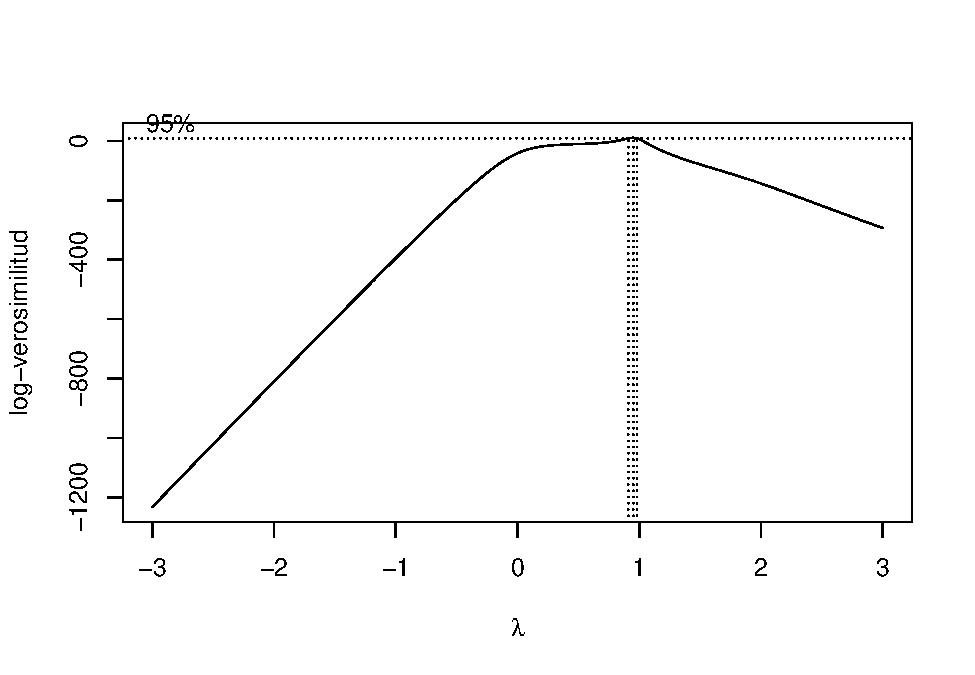
\includegraphics{Taller-2-Regresion-Multiple-Aplicada_files/figure-latex/unnamed-chunk-5-1.pdf}

\begin{verbatim}
## [1] "Shapiro Test; H0: Normalidad vs H1: No Normalidad"
## 
##  Shapiro-Wilk normality test
## 
## data:  studres(model)
## W = 0.86458, p-value = 0.001868
## 
## [1] "Breusch Pagan Test;H0: Homocedasticidad vs H1: No Homocedasticidad"
## 
##  studentized Breusch-Pagan test
## 
## data:  model
## BP = 27.288, df = 24, p-value = 0.2912
\end{verbatim}

Mediante el grafico y los valores P asociados a la homocedasticidad y
normalidad de residuos se evidencia el incumplimiento de la normalidad
de los residuos.

\begin{Shaded}
\begin{Highlighting}[]
\FunctionTok{hist}\NormalTok{(}\FunctionTok{studres}\NormalTok{(model),}\AttributeTok{lwd=}\DecValTok{2}\NormalTok{,}\AttributeTok{col=}\StringTok{\textquotesingle{}aquamarine4\textquotesingle{}}\NormalTok{,}\AttributeTok{freq=}\NormalTok{F,}\AttributeTok{ylim=}\FunctionTok{c}\NormalTok{(}\DecValTok{0}\NormalTok{,}\FloatTok{0.4}\NormalTok{),}
     \AttributeTok{xlab=}\StringTok{\textquotesingle{}Residuos Estudentizados Modelo\textquotesingle{}}\NormalTok{,}\AttributeTok{main=}\StringTok{\textquotesingle{}\textquotesingle{}}\NormalTok{)}
\FunctionTok{lines}\NormalTok{(}\FunctionTok{density}\NormalTok{(}\FunctionTok{studres}\NormalTok{(model)),}\AttributeTok{lwd=}\DecValTok{2}\NormalTok{,}\AttributeTok{col=}\StringTok{\textquotesingle{}black\textquotesingle{}}\NormalTok{)}
\end{Highlighting}
\end{Shaded}

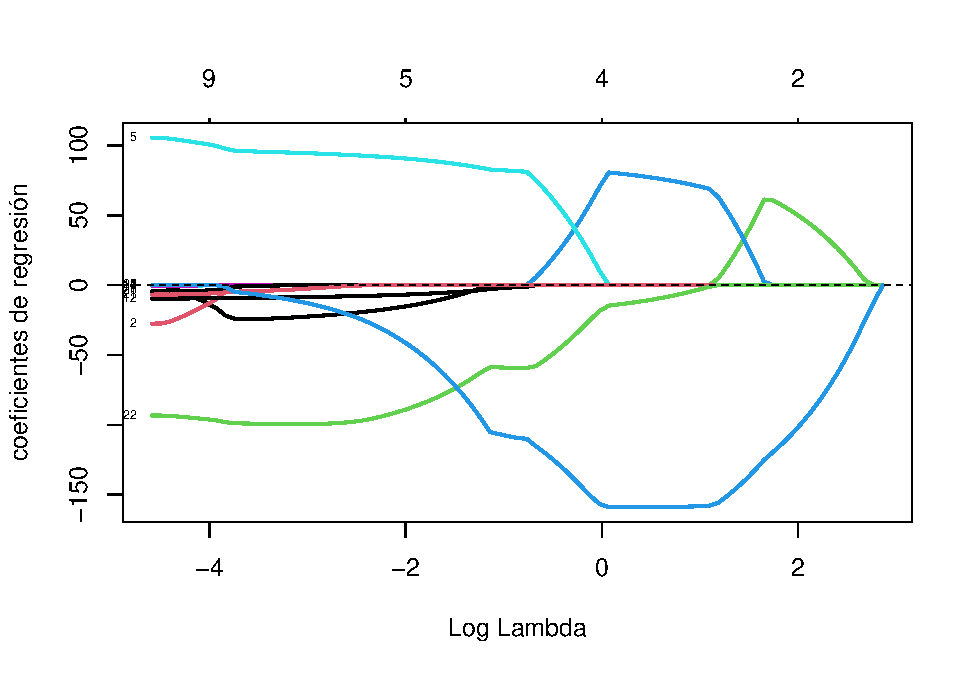
\includegraphics{Taller-2-Regresion-Multiple-Aplicada_files/figure-latex/unnamed-chunk-6-1.pdf}

Como no se cumple el supuesto de normalidad se procede a corregir
mediante el metodo de BoxCox y se verifica el cumplimiento de los
mismos.

\begin{Shaded}
\begin{Highlighting}[]
\NormalTok{model }\OtherTok{\textless{}{-}} \FunctionTok{lm}\NormalTok{(density}\FloatTok{+0.01} \SpecialCharTok{\textasciitilde{}}\NormalTok{ .}\SpecialCharTok{{-}}\NormalTok{NIR1}\SpecialCharTok{{-}}\NormalTok{NIR8}\SpecialCharTok{{-}}\NormalTok{NIR9}\SpecialCharTok{{-}}\NormalTok{NIR10}\SpecialCharTok{{-}}\NormalTok{NIR11}\SpecialCharTok{{-}}\NormalTok{NIR7, }\AttributeTok{data=}\NormalTok{X)}
\FunctionTok{lambda}\NormalTok{(model,}\FloatTok{0.5}\NormalTok{,}\FloatTok{1.5}\NormalTok{)}
\end{Highlighting}
\end{Shaded}

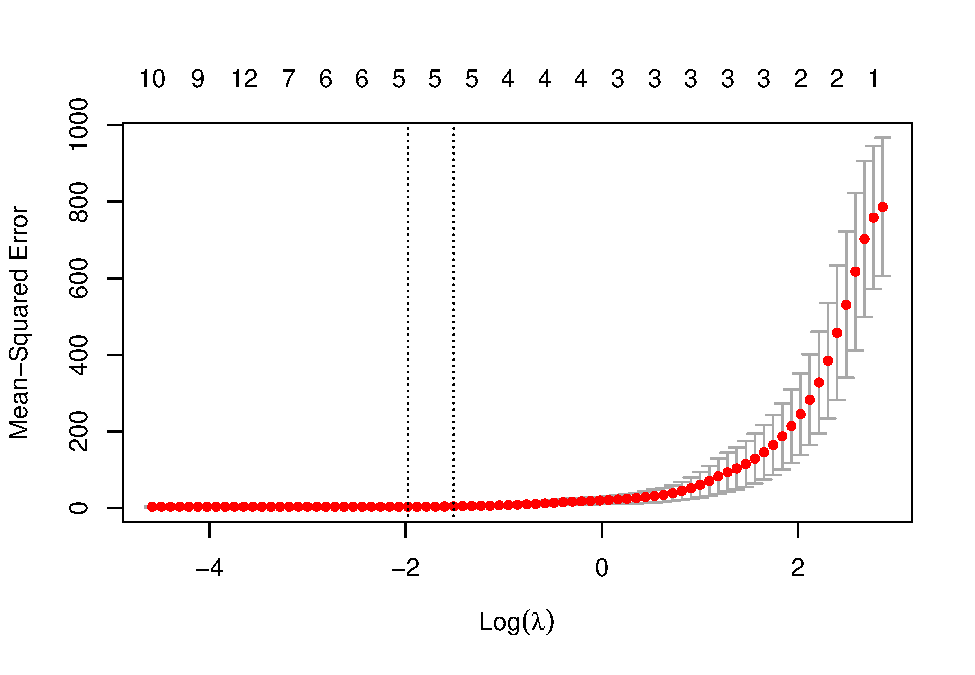
\includegraphics{Taller-2-Regresion-Multiple-Aplicada_files/figure-latex/unnamed-chunk-7-1.pdf}

\begin{verbatim}
## [1] 0.97
\end{verbatim}

\begin{Shaded}
\begin{Highlighting}[]
\NormalTok{model.box }\OtherTok{\textless{}{-}} \FunctionTok{lm}\NormalTok{(}\FunctionTok{I}\NormalTok{(density}\SpecialCharTok{\^{}}\FloatTok{0.96}\NormalTok{) }\SpecialCharTok{\textasciitilde{}}\NormalTok{.}\SpecialCharTok{{-}}\NormalTok{NIR1}\SpecialCharTok{{-}}\NormalTok{NIR8}\SpecialCharTok{{-}}\NormalTok{NIR9}\SpecialCharTok{{-}}\NormalTok{NIR10}\SpecialCharTok{{-}}\NormalTok{NIR11}\SpecialCharTok{{-}}\NormalTok{NIR7,}\AttributeTok{data=}\NormalTok{X)}
\FunctionTok{validaciongrafica}\NormalTok{(model.box)}
\end{Highlighting}
\end{Shaded}

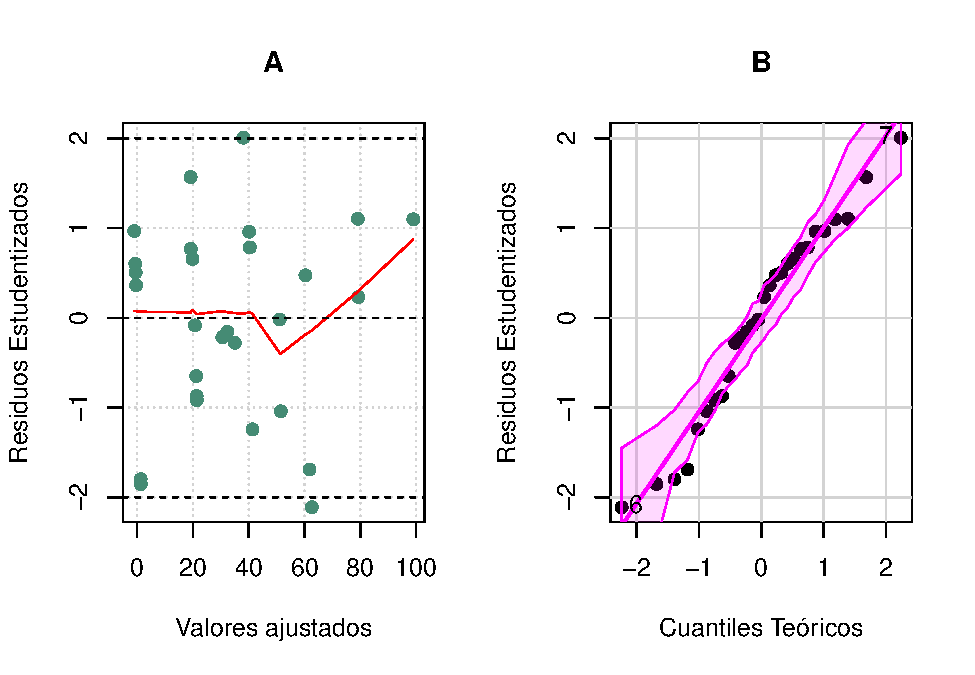
\includegraphics{Taller-2-Regresion-Multiple-Aplicada_files/figure-latex/unnamed-chunk-8-1.pdf}
{[}1{]} ``Shapiro Test; H0: Normalidad vs H1: No Normalidad''

\begin{verbatim}
Shapiro-Wilk normality test
\end{verbatim}

data: studres(model) W = 0.97774, p-value = 0.7934

{[}1{]} ``Breusch Pagan Test;H0: Homocedasticidad vs H1: No
Homocedasticidad''

\begin{verbatim}
studentized Breusch-Pagan test
\end{verbatim}

data: model BP = 23.94, df = 24, p-value = 0.4651

Mediante el grafico y los valores P asociados a la homocedasticidad y
normalidad de residuos se evidencia el cumplimiento de ambos supuestos.

\begin{Shaded}
\begin{Highlighting}[]
\FunctionTok{hist}\NormalTok{(}\FunctionTok{studres}\NormalTok{(model.box),}\AttributeTok{lwd=}\DecValTok{2}\NormalTok{,}\AttributeTok{col=}\StringTok{\textquotesingle{}aquamarine4\textquotesingle{}}\NormalTok{,}
\AttributeTok{freq=}\NormalTok{F,}\AttributeTok{ylim=}\FunctionTok{c}\NormalTok{(}\DecValTok{0}\NormalTok{,}\FloatTok{0.4}\NormalTok{),}\AttributeTok{xlab=}\StringTok{\textquotesingle{}Residuos Estudentizados Modelo\textquotesingle{}}\NormalTok{,}\AttributeTok{main=}\StringTok{\textquotesingle{}\textquotesingle{}}\NormalTok{)}
\FunctionTok{lines}\NormalTok{(}\FunctionTok{density}\NormalTok{(}\FunctionTok{studres}\NormalTok{(model.box)),}\AttributeTok{lwd=}\DecValTok{2}\NormalTok{,}\AttributeTok{col=}\StringTok{\textquotesingle{}black\textquotesingle{}}\NormalTok{)}
\end{Highlighting}
\end{Shaded}

\includegraphics{Taller-2-Regresion-Multiple-Aplicada_files/figure-latex/unnamed-chunk-9-1.pdf}

Ya con los requerimentos necesarios para realizar regresión de LASSO se
procede a calcular el valor de \(\lambda\) optimo mediante la validación
cruzada

\hypertarget{validaciuxf3n-cruzada}{%
\subsubsection{Validación cruzada}\label{validaciuxf3n-cruzada}}

Es un método para evaluar que tan bueno es un modelo para predecir
observaciones futuras de la población objeto de estudio. La muestra se
divide en dos grupos:

\begin{itemize}
\item
  Entrenamiento: Se usa para ajustar el modelo.
\item
  Validación: Se utiliza para validar el modelo ajustado.
\end{itemize}

Se realiza K interacciones dividiendo los datos en K subconjuntos. En
cada interacción uno de los subconjuntos es utilizado para validación,
el el resto (K-1) como datos de entrenamiento. Para cada división,
k=1,..,k y para cada valor de \(\lambda\) se estima el modelo basado en
la muestra de entrenamiento. Mientras que con cada muestra de validación
y para cada valor de \(\lambda\) se utiliza para calcular el error
cuadratico medio:

\[ECM_k(\lambda)= \sum_{i=1}^{n_k}\frac{(y_i^k- x_i^k*\hat{\beta}^k(\lambda))^2}{n}\]

Donde \(y_i^k\) son las observaciones de la muestra de validación k y
\(\hat{\beta}^k\) es la estimacion utilizando la muestra de
entrenamiento k. para cada \(\lambda\) se calcula:

\(CV(\lambda)=\frac{1}{k}\sum_{i=1}^{K}ECM_k(\lambda)\)

Y la desviación estándar:

\(SD(\lambda)=\sqrt{\sum_{i=1}^{K}\frac{(ECM_k(\lambda)-CV(\lambda))^2}{K-1}}\)

\(\lambda\) optimo: minimiza \(CV{\lambda}\) o

maximiza \(\lambda\):
\(CV(\hat{\lambda}) < CV(\hat{\lambda}_{cv})+SD(\hat{\lambda}_{cv})\)

La maximisación es mas optima ya que se tiene en cuenta la variabilidad
debida a la selección de las submuestras.

\begin{Shaded}
\begin{Highlighting}[]
\NormalTok{X.}\OtherTok{\textless{}{-}}\FunctionTok{model.matrix}\NormalTok{(model.box)[,}\SpecialCharTok{{-}}\DecValTok{1}\NormalTok{]}
\NormalTok{lasso.cv }\OtherTok{\textless{}{-}}\FunctionTok{cv.glmnet}\NormalTok{(X., X}\SpecialCharTok{$}\NormalTok{density, }\AttributeTok{nfolds =} \DecValTok{4}\NormalTok{, }\AttributeTok{alpha =} \DecValTok{1}\NormalTok{,}
                     \AttributeTok{nlambda =} \DecValTok{100}\NormalTok{)}
\FunctionTok{plot}\NormalTok{(lasso.cv)}
\end{Highlighting}
\end{Shaded}

\includegraphics{Taller-2-Regresion-Multiple-Aplicada_files/figure-latex/unnamed-chunk-10-1.pdf}

\begin{Shaded}
\begin{Highlighting}[]
\NormalTok{est }\OtherTok{=} \FunctionTok{glmnet}\NormalTok{(X., X}\SpecialCharTok{$}\NormalTok{density, }\AttributeTok{alpha =} \DecValTok{1}\NormalTok{,}\AttributeTok{lambda =}\NormalTok{ lasso.cv}\SpecialCharTok{$}\NormalTok{lambda}\FloatTok{.1}\NormalTok{se)}
\NormalTok{est}\SpecialCharTok{$}\NormalTok{beta}
\end{Highlighting}
\end{Shaded}

\begin{verbatim}
## 24 x 1 sparse Matrix of class "dgCMatrix"
##               s0
## NIR2   -6.712815
## NIR3    .       
## NIR4    .       
## NIR5    .       
## NIR6   86.161212
## NIR12   .       
## NIR13   .       
## NIR14   .       
## NIR15   .       
## NIR16   .       
## NIR17   .       
## NIR18  -4.484754
## NIR19   .       
## NIR20   .       
## NIR21   .       
## NIR22   .       
## NIR23   .       
## NIR24   .       
## NIR25   .       
## NIR26   .       
## NIR27   .       
## NIR28 -88.761674
## NIR29 -49.934344
## NIR30   .
\end{verbatim}

La selección de variables por medio del estimador LASSO son: NIR2, NIR6,
NIR18, NIR28, NIR29. Veremos el resumen del modelo para evaluar las
pruebas individuales t a ver si podemos considerar descartar alguna
covariable adicional. Cabe aclarar que a pesar de haber realizado la
selección de variables, no podemos dejarlo todo a los métodos sino por
el contrario seguir indagando e intetando llegar al mejor modelo
posible.

\begin{Shaded}
\begin{Highlighting}[]
\NormalTok{model.lasso1 }\OtherTok{\textless{}{-}} \FunctionTok{lm}\NormalTok{(density}\SpecialCharTok{\textasciitilde{}}\NormalTok{NIR2}\SpecialCharTok{+}\NormalTok{NIR6}\SpecialCharTok{+}\NormalTok{NIR18}\SpecialCharTok{+}\NormalTok{NIR28}\SpecialCharTok{+}\NormalTok{NIR29,}\AttributeTok{data=}\NormalTok{X)}
\FunctionTok{summary}\NormalTok{(model.lasso1)}
\end{Highlighting}
\end{Shaded}

\begin{verbatim}
## 
## Call:
## lm(formula = density ~ NIR2 + NIR6 + NIR18 + NIR28 + NIR29, data = X)
## 
## Residuals:
##      Min       1Q   Median       3Q      Max 
## -1.99054 -0.86304  0.07117  0.81460  1.63877 
## 
## Coefficients:
##             Estimate Std. Error t value Pr(>|t|)    
## (Intercept)   20.808     15.525   1.340 0.193832    
## NIR2         -27.826      4.424  -6.290 2.49e-06 ***
## NIR6          96.932      2.036  47.615  < 2e-16 ***
## NIR18         -9.649      2.071  -4.659 0.000121 ***
## NIR28       -123.484     18.545  -6.659 1.08e-06 ***
## NIR29         24.496     31.814   0.770 0.449495    
## ---
## Signif. codes:  0 '***' 0.001 '**' 0.01 '*' 0.05 '.' 0.1 ' ' 1
## 
## Residual standard error: 1.18 on 22 degrees of freedom
## Multiple R-squared:  0.9984, Adjusted R-squared:  0.9981 
## F-statistic:  2817 on 5 and 22 DF,  p-value: < 2.2e-16
\end{verbatim}

Consiguiente a eso se procede a realizar una prueba sobre subconjuntos
para evaluar si podemos eliminar NIR29 para disminuir problemas de
multicolinealidad.

\hypertarget{suma-extra-de-cuadrados}{%
\subsection{Suma extra de cuadrados}\label{suma-extra-de-cuadrados}}

Sirve para probar la significancia de un subconjunto de coeficientes.

Se tiene el siguiente modelo:

\[y = X\beta+\varepsilon\] donde
\(\beta\)=\(\begin{bmatrix} \beta_{1}\\ \beta_{2} \\ \end{bmatrix}\)

donde \(\beta_1\) es un vector (p-r)x1 y \(\beta_2\) es un vector rx1 ,
se quiere evaluar la siguiente hipotesis:

\begin{center}
$H_0 : \beta_2 =0$ vs $H_1: \beta_2 \neq 0 $
\end{center}

Se tienen los siguientes modelos: Modelo completo :
\(y = X_1\beta_1+X_2\beta_2+\varepsilon\)

\(SCR(B)= y^T(H-\frac{1}{n}11^T)y\)

Modelo reducido : \(y = X_1\beta_1\varepsilon\)

\(SCR(B_1)= y^T(H_1-\frac{1}{n}11^T)y\)

La suma de cuadrados de la regresión debida a \(\beta_2\) dado que
\(\beta_1\) ya esta en el modelo es:
\[SSR(\beta_2|\beta_1)=SSR(\beta)-SSR(\beta_1)\] Conocida como suma
extra de cuadrados debido a \(\beta_2\), y dado que queremos probar
\(H_0 : \beta_2 =0\) se construye el siguiente estadistico.

\(F_0 = \frac{\frac{SSR(\beta_2|\beta_1)}{r}}{\frac{SE}{n-p}}\)

Si \(H_0\) es cierta entonces \(F_0\) \textasciitilde{} \(F_{r,n-p}\)

Se realiza la respectiva prueba con la funcion anova, asumiento que el
modelo reducido es aquel \(\beta_5\)=0 asociado al NIR29

Hipotesis: \(H_0:\beta_5=0\) VS \(H_1:\beta_5\neq0\)

\begin{Shaded}
\begin{Highlighting}[]
\NormalTok{model.lasso1 }\OtherTok{\textless{}{-}} \FunctionTok{lm}\NormalTok{(density}\SpecialCharTok{\textasciitilde{}}\NormalTok{NIR2}\SpecialCharTok{+}\NormalTok{NIR6}\SpecialCharTok{+}\NormalTok{NIR18}\SpecialCharTok{+}\NormalTok{NIR28}\SpecialCharTok{+}\NormalTok{NIR29,}\AttributeTok{data=}\NormalTok{X)}
\NormalTok{model.lasso2 }\OtherTok{\textless{}{-}} \FunctionTok{lm}\NormalTok{(density}\SpecialCharTok{\textasciitilde{}}\NormalTok{NIR2}\SpecialCharTok{+}\NormalTok{NIR6}\SpecialCharTok{+}\NormalTok{NIR18}\SpecialCharTok{+}\NormalTok{NIR28,}\AttributeTok{data=}\NormalTok{X)}
\FunctionTok{anova}\NormalTok{(model.lasso2,model.lasso1)}
\end{Highlighting}
\end{Shaded}

\begin{verbatim}
## Analysis of Variance Table
## 
## Model 1: density ~ NIR2 + NIR6 + NIR18 + NIR28
## Model 2: density ~ NIR2 + NIR6 + NIR18 + NIR28 + NIR29
##   Res.Df    RSS Df Sum of Sq      F Pr(>F)
## 1     23 31.435                           
## 2     22 30.610  1   0.82493 0.5929 0.4495
\end{verbatim}

La prueba anova indica un valor P de 0.4495 lo que indica que el
coeficiente asociado al NIR29 es significativamente 0, por ende, podemos
retirarlo del modelo ya que no aporta a la estimación de la densidad y
en cambio aumenta el VIF como se evidencia acontinuación.

\hypertarget{factor-de-inflaciuxf3n-de-varianza-vif}{%
\subsection{Factor de inflación de varianza
(VIF)}\label{factor-de-inflaciuxf3n-de-varianza-vif}}

Es una medida que detecta si hay problemas de multicolinealidad.
Generalmente un VIF mayor a 10 indica problemas graves de
multicolinealidad.

\(VIF_j = \frac{1}{1-R^2}\)

Donde \(R^2_j\) es el coeficiente de determinación obtenido ajustando
una regresión de \(x_j\) sobre las demás covariables.

\(VIF_j = \sum_{j=1}^{p-1}\frac{t^2_{ij}}{\lambda_j}\)

Donde \(T=(t_1,....,t_{p-1})\) es una matriz ortogonal de vectores
propios y \(\lambda_j\) los valores propios asociados a la
descomposición de la matriz \(R=Z^TZ\) y Z es la matrix de X
estandarizada. \(R=TAT^T\) (descomposición)

\begin{Shaded}
\begin{Highlighting}[]
\NormalTok{car}\SpecialCharTok{::}\FunctionTok{vif}\NormalTok{(model.lasso1)}
\end{Highlighting}
\end{Shaded}

\begin{verbatim}
##       NIR2       NIR6      NIR18      NIR28      NIR29 
##   3.766765   5.643206  36.089199 269.277707 304.968458
\end{verbatim}

\begin{Shaded}
\begin{Highlighting}[]
\NormalTok{car}\SpecialCharTok{::}\FunctionTok{vif}\NormalTok{(model.lasso2)}
\end{Highlighting}
\end{Shaded}

\begin{verbatim}
##      NIR2      NIR6     NIR18     NIR28 
##  2.967327  4.203285 31.085734 26.983026
\end{verbatim}

\hypertarget{modelo-de-regresiuxf3n-multiple}{%
\section{Modelo de regresión
multiple}\label{modelo-de-regresiuxf3n-multiple}}

Con base en el proceso de selección de variables se ajusta el siguiente
modelo y se realiza la respectiva validación de supuestos:

\begin{Shaded}
\begin{Highlighting}[]
\NormalTok{model.lasso1}\OtherTok{\textless{}{-}} \FunctionTok{lm}\NormalTok{(density}\SpecialCharTok{\textasciitilde{}}\NormalTok{NIR2}\SpecialCharTok{+}\NormalTok{NIR6}\SpecialCharTok{+}\NormalTok{NIR18}\SpecialCharTok{+}\NormalTok{NIR28,}\AttributeTok{data=}\NormalTok{X)}
\FunctionTok{summary}\NormalTok{(model.lasso1)}
\end{Highlighting}
\end{Shaded}

\begin{verbatim}
## 
## Call:
## lm(formula = density ~ NIR2 + NIR6 + NIR18 + NIR28, data = X)
## 
## Residuals:
##     Min      1Q  Median      3Q     Max 
## -2.1312 -0.9776  0.1102  0.8381  2.0416 
## 
## Coefficients:
##             Estimate Std. Error t value Pr(>|t|)    
## (Intercept)   29.389     10.712   2.744   0.0116 *  
## NIR2         -26.257      3.892  -6.747 6.99e-07 ***
## NIR6          96.140      1.741  55.211  < 2e-16 ***
## NIR18         -9.055      1.905  -4.753 8.62e-05 ***
## NIR28       -109.939      5.818 -18.896 1.66e-15 ***
## ---
## Signif. codes:  0 '***' 0.001 '**' 0.01 '*' 0.05 '.' 0.1 ' ' 1
## 
## Residual standard error: 1.169 on 23 degrees of freedom
## Multiple R-squared:  0.9984, Adjusted R-squared:  0.9981 
## F-statistic:  3584 on 4 and 23 DF,  p-value: < 2.2e-16
\end{verbatim}

\hypertarget{interpretaciuxf3n}{%
\subsection{Interpretación}\label{interpretaciuxf3n}}

\begin{itemize}
\item
  En el resumen del modelo contamos con un \(R^2=0.9984\), es decir, el
  99.84 de la variabilidad de la densidad del Hilo PET está siendo
  explicada por el modelo. Se cuenta con un \(R^2_{adj}\) de 0.9981.
\item
  El valor del estadístico F es de 3584 con un valor p asociado de
  aproximadamente 0 lo que indica que por lo menos una de estas
  estimaciones de los \(\beta_i\) es diferente de 0. Por ende ajustar el
  modelo ayuda a la predicción de la densidad del Hilo de Pet.
\item
  Observamos relaciones negativas entre la densidad y el conjunto de
  covariables NIR2, NIR 18 y NIR28 SI asumimos que se presentan aumentos
  con las demas covariables constantes, y se presenta una relación
  positiva entre la densidad y el NIR6 si mantenemos las demas
  covariables constantes.
\end{itemize}

\hypertarget{anova}{%
\paragraph{ANOVA}\label{anova}}

\begin{Shaded}
\begin{Highlighting}[]
\FunctionTok{Anova}\NormalTok{(model.lasso1)}
\end{Highlighting}
\end{Shaded}

\begin{verbatim}
## Anova Table (Type II tests)
## 
## Response: density
##           Sum Sq Df  F value    Pr(>F)    
## NIR2        62.2  1   45.520 6.995e-07 ***
## NIR6      4166.2  1 3048.258 < 2.2e-16 ***
## NIR18       30.9  1   22.591 8.615e-05 ***
## NIR28      488.0  1  357.056 1.661e-15 ***
## Residuals   31.4 23                       
## ---
## Signif. codes:  0 '***' 0.001 '**' 0.01 '*' 0.05 '.' 0.1 ' ' 1
\end{verbatim}

La tabla ANOVA realiza pruebas sobre subconjuntos de coeficientes
haciendo uso de la suma de cuadrados extra.

Estadistico F asociado al NIR2 :
\(F_0 = \frac{{SSR(\beta_1|\beta_0)}}{\frac{SE}{26}}\)

Modelo: \(y =\beta_0+NIR2\beta_1+\varepsilon\)

Hipotesis: \(H_0: \beta_1=0\)

Estadistico F asociado al NIR6 :
\(F_0 = \frac{{SSR(\beta_2|\beta_1,\beta_0)}}{\frac{SE}{26}}\)

Modelo: \(y =\beta_0+NIR2\beta_1+NIR6\beta_2+\varepsilon\)

Hipotesis: \(H_0: \beta_2=0\)

Estadistico F asociado al NIR18 :
\(F_0 = \frac{{SSR(\beta_3|\beta_0,\beta_1,\beta_2)}}{\frac{SE}{26}}\)

Modelo: \(y =\beta_0+NIR2\beta_1+NIR6\beta_2+NIR18\beta_3+\varepsilon\)

Hipotesis: \(H_0: \beta_3=0\)

En cada hipoteis evaluada el valor p es menor a un nivel de
significancia al 5\% lo que indica que para cada caso, añadir el
\(\beta_i\) es significativamente distinto de 0

\hypertarget{validaciuxf3n-de-supuestos}{%
\subsection{Validación de supuestos}\label{validaciuxf3n-de-supuestos}}

\begin{Shaded}
\begin{Highlighting}[]
\FunctionTok{validaciongrafica}\NormalTok{(model.lasso1)}
\end{Highlighting}
\end{Shaded}

\includegraphics{Taller-2-Regresion-Multiple-Aplicada_files/figure-latex/unnamed-chunk-16-1.pdf}

\begin{verbatim}
## [1] "Shapiro Test; H0: Normalidad vs H1: No Normalidad"
## 
##  Shapiro-Wilk normality test
## 
## data:  studres(model)
## W = 0.96468, p-value = 0.4471
## 
## [1] "Breusch Pagan Test;H0: Homocedasticidad vs H1: No Homocedasticidad"
## 
##  studentized Breusch-Pagan test
## 
## data:  model
## BP = 1.6317, df = 4, p-value = 0.8031
\end{verbatim}

\begin{Shaded}
\begin{Highlighting}[]
\FunctionTok{hist}\NormalTok{(}\FunctionTok{studres}\NormalTok{(model.lasso1),}\AttributeTok{lwd=}\DecValTok{2}\NormalTok{,}\AttributeTok{col=}\StringTok{\textquotesingle{}aquamarine4\textquotesingle{}}\NormalTok{,}
\AttributeTok{freq=}\NormalTok{F,}\AttributeTok{ylim=}\FunctionTok{c}\NormalTok{(}\DecValTok{0}\NormalTok{,}\FloatTok{0.4}\NormalTok{),}\AttributeTok{xlab=}\StringTok{\textquotesingle{}Residuos Estudentizados Modelo\textquotesingle{}}\NormalTok{,}\AttributeTok{main=}\StringTok{\textquotesingle{}\textquotesingle{}}\NormalTok{)}
\FunctionTok{lines}\NormalTok{(}\FunctionTok{density}\NormalTok{(}\FunctionTok{studres}\NormalTok{(model.lasso1)),}\AttributeTok{lwd=}\DecValTok{2}\NormalTok{,}\AttributeTok{col=}\StringTok{\textquotesingle{}black\textquotesingle{}}\NormalTok{)}
\end{Highlighting}
\end{Shaded}

\includegraphics{Taller-2-Regresion-Multiple-Aplicada_files/figure-latex/unnamed-chunk-17-1.pdf}

Como se evidencia en los graficos y en las pruebas formales, ambos
coinciden con sus respectivos resultados, es decir, varianza constante
(Homocedasticidad) y distribución Normal en los errores.

\hypertarget{identificaciuxf3n-de-puntosa-atuxedpicos-e-influyentes}{%
\subsection{Identificación de puntosa atípicos e
influyentes}\label{identificaciuxf3n-de-puntosa-atuxedpicos-e-influyentes}}

Para esto utilizaremos la función influence.measures()

\begin{Shaded}
\begin{Highlighting}[]
\FunctionTok{influence.measures}\NormalTok{(model.lasso1)}
\end{Highlighting}
\end{Shaded}

\begin{verbatim}
## Influence measures of
##   lm(formula = density ~ NIR2 + NIR6 + NIR18 + NIR28, data = X) :
## 
##      dfb.1_  dfb.NIR2  dfb.NIR6 dfb.NIR1 dfb.NIR28    dffit cov.r   cook.d
## 1   0.14096 -0.373395  0.649685 -0.33177   0.18411  0.82826 1.500 1.36e-01
## 2   0.27322 -0.305493  0.372058  0.07340  -0.15731  0.55437 1.194 6.09e-02
## 3  -0.02220 -0.019232  0.075059 -0.08171   0.06129  0.12878 1.614 3.46e-03
## 4   0.14484 -0.106548  0.083888  0.14236  -0.15812  0.23851 1.488 1.18e-02
## 5  -0.08091  0.074553 -0.179345 -0.04769   0.11805 -0.49216 0.735 4.48e-02
## 6   0.28982 -0.191413 -0.085880  0.40391  -0.28227 -0.86071 0.579 1.29e-01
## 7   0.25096 -0.167777  0.160191  0.43368  -0.40108  0.82045 0.629 1.19e-01
## 8  -0.05430 -0.069031  0.088418 -0.26894   0.26591 -0.39673 0.979 3.07e-02
## 9  -0.31667  0.306438 -0.157325 -0.13253   0.13285  0.37797 1.341 2.91e-02
## 10 -0.25575  0.271697 -0.198103 -0.17086   0.14730  0.46733 1.258 4.38e-02
## 11  0.09966 -0.157527  0.149988  0.00659   0.01782  0.29877 1.369 1.83e-02
## 12 -0.11748  0.038782  0.043501 -0.21867   0.18849 -0.32619 1.201 2.15e-02
## 13  0.03205 -0.131950  0.183335 -0.15597   0.12961 -0.28270 1.133 1.61e-02
## 14  0.00823 -0.016193  0.021363 -0.00371   0.00259 -0.02852 1.391 1.70e-04
## 15 -0.09547  0.157450 -0.316257 -0.20703   0.19369  0.75836 0.907 1.08e-01
## 16  0.95360  0.170445 -0.962860  1.79595  -1.99192 -2.33670 1.566 9.88e-01
## 17 -0.05625 -0.012588  0.045322 -0.09968   0.12613  0.19576 1.564 7.96e-03
## 18 -0.00244 -0.003507 -0.038110  0.00356   0.03279  0.20992 1.290 9.06e-03
## 19  0.11085 -0.061830 -0.111279  0.06139  -0.01992  0.34215 1.141 2.35e-02
## 20  0.14056 -0.100783 -0.051670  0.03438  -0.02407  0.25630 1.485 1.36e-02
## 21 -1.63766  1.547939 -0.334048 -0.01507   0.06714 -2.26423 1.624 9.34e-01
## 22  0.00023 -0.000734 -0.000306 -0.00120   0.00153 -0.00471 1.329 4.64e-06
## 23  0.02319 -0.062385  0.020799 -0.04146   0.06834 -0.26223 1.044 1.37e-02
## 24  0.00721 -0.019265  0.017150 -0.02612   0.02270 -0.04970 1.368 5.16e-04
## 25  0.03863 -0.065311  0.056280 -0.03468   0.03119 -0.09300 1.363 1.80e-03
## 26  0.02213 -0.046422  0.053056 -0.02059   0.01966 -0.07220 1.372 1.09e-03
## 27 -0.05245  0.009424  0.035150 -0.11578   0.09533 -0.20031 1.244 8.23e-03
## 28 -0.15921  0.213025 -0.202562  0.01841   0.00497  0.27478 1.234 1.54e-02
##       hat inf
## 1  0.3624    
## 2  0.2014    
## 3  0.2358    
## 4  0.2022    
## 5  0.0781    
## 6  0.1425    
## 7  0.1432    
## 8  0.0923    
## 9  0.1885    
## 10 0.1916    
## 11 0.1718    
## 12 0.1227    
## 13 0.0866    
## 14 0.1033    
## 15 0.1895    
## 16 0.6139   *
## 17 0.2252    
## 18 0.1083    
## 19 0.1111    
## 20 0.2058    
## 21 0.6130   *
## 22 0.0601    
## 23 0.0595    
## 24 0.0918    
## 25 0.0998    
## 26 0.0995    
## 27 0.0868    
## 28 0.1133
\end{verbatim}

\begin{Shaded}
\begin{Highlighting}[]
\CommentTok{\#Puntos de Balanceo, Influyentes y Atípicos}
\FunctionTok{par}\NormalTok{(}\AttributeTok{mfrow=}\FunctionTok{c}\NormalTok{(}\DecValTok{1}\NormalTok{,}\DecValTok{1}\NormalTok{))}
\FunctionTok{influencePlot}\NormalTok{(model.lasso1,}\AttributeTok{panel.first=}\FunctionTok{grid}\NormalTok{(),}\AttributeTok{ylab=}\StringTok{\textquotesingle{}Residuos Studentizados\textquotesingle{}}\NormalTok{)}
\end{Highlighting}
\end{Shaded}

\includegraphics{Taller-2-Regresion-Multiple-Aplicada_files/figure-latex/unnamed-chunk-18-1.pdf}

\begin{verbatim}
##      StudRes       Hat     CookD
## 6  -2.111444 0.1424941 0.1288001
## 7   2.006935 0.1431940 0.1189678
## 16 -1.853127 0.6138988 0.9875246
## 21 -1.799176 0.6129686 0.9344561
\end{verbatim}

Dónde observamos que las observaciones 16,21 son influyentes a nuestro
modelo y las 6,7 atípicas. Los puntos dentro de la base de datos lucen
así y procedemos a ilustrarlos para que cuando un experto en el tema
pueda considerarlos y evaluar si fueron errores de mediciones o que
ocurre realmente con ellos. A su vez mostraremos los efectos de cada
covariable con densidad. En general observamos que la relación de NIR2,
18 y 28 describen relaciones lineales negativas, inversamente
proporcionales, a diferencia de la relación con NIR6 que es positiva,
directamente proporcional.

\begin{Shaded}
\begin{Highlighting}[]
\NormalTok{X[}\FunctionTok{c}\NormalTok{(}\DecValTok{6}\NormalTok{,}\DecValTok{7}\NormalTok{,}\DecValTok{16}\NormalTok{,}\DecValTok{21}\NormalTok{),}\FunctionTok{c}\NormalTok{(}\DecValTok{2}\NormalTok{,}\DecValTok{6}\NormalTok{,}\DecValTok{18}\NormalTok{,}\DecValTok{28}\NormalTok{,}\DecValTok{31}\NormalTok{)]}
\end{Highlighting}
\end{Shaded}

\begin{verbatim}
##      NIR2   NIR6  NIR18  NIR28 density
## 6  3.0849 2.5089 1.1999 1.0562   60.48
## 7  3.1372 2.9268 2.8934 1.4930   40.10
## 16 3.1229 2.9345 3.3254 1.8021    0.00
## 21 2.6803 1.8602 1.3031 1.1352    0.00
\end{verbatim}

\begin{Shaded}
\begin{Highlighting}[]
\FunctionTok{plot}\NormalTok{(}\FunctionTok{allEffects}\NormalTok{(model.lasso1))}
\end{Highlighting}
\end{Shaded}

\includegraphics{Taller-2-Regresion-Multiple-Aplicada_files/figure-latex/unnamed-chunk-19-1.pdf}

Generamos una predicción con el modelo seleccionado:

\begin{Shaded}
\begin{Highlighting}[]
\NormalTok{x.nuevo}\OtherTok{\textless{}{-}} \FunctionTok{data.frame}\NormalTok{(}\AttributeTok{NIR2=}\FloatTok{3.06}\NormalTok{,}\AttributeTok{NIR6=}\FloatTok{2.55}\NormalTok{,}\AttributeTok{NIR18=}\FloatTok{2.14}\NormalTok{,}\AttributeTok{NIR28=}\FloatTok{1.32}\NormalTok{)}
\NormalTok{pred.media }\OtherTok{=} \FunctionTok{predict}\NormalTok{(model.lasso1,x.nuevo,}\AttributeTok{interval =} \StringTok{"confidence"}\NormalTok{)}
\NormalTok{pred.media}
\end{Highlighting}
\end{Shaded}

\begin{verbatim}
##        fit      lwr      upr
## 1 29.70163 29.21701 30.18625
\end{verbatim}

\hypertarget{regresiuxf3n-ridge}{%
\section{Regresión ridge}\label{regresiuxf3n-ridge}}

A pesar de que evidenciamos claras mejoras en los problemas de
multicolinealidad dada la selección de variables, procederemos a
realizar la regresión de ridge que tiene como objetivo minimizar la
siguiente suma de cuadrados penalizada:

\begin{center}
$S_{k}(\beta)=\sum_{i=1}^{n}({y_{i}-z^
T}\beta)^2+k\sum_{j=1}^{p-1}\beta^2_{j}$
\end{center}

Al realizar derivada e igualar a 0 se obtienen las siguiente estimación:

\[\hat{\beta}_{k}= (R+kI)^{-1}Z^Ty\] Donde:
\[E(\hat{\beta}_{k})=E((I+kR^{-1})^{-1}\hat{\beta})=C\beta\]

y \[V(\hat{\beta}_{k})=\sigma^2C^{T}R^{-1}C\]

Por ultimo se calcula el error cuadrático medio de \(\hat{\beta_k}\)

\[ECM(\hat{\beta_k})=trV(\hat{\beta_k})+(E(\hat{\beta_k})-\beta)^t(E(\hat{\beta_k})-\beta)\]
\[=\sigma^2tr(R^{-1}C^TC)+\beta^T(C-I)^T(C-I)\beta\]
\[=\sigma^2\sum_{i=1}^{p-1}\frac{\lambda_j}{(\lambda_j+k)^2}+\sum_{i=1}^{p-1}\frac{\alpha^2_jk^2}{(\lambda_j+k)^2}\]
Se observa que si k crece, disminuye la varianza, pero aumenta el sesgo.
Por lo que la idea es obtener un k que minimize el ECM.

Luego de tener claro estos conceptos procedemos a realizar la regresión
de ridge utilizando la librería lmridge. Para poder realizar esto
generamos una secuencia de 1000 valores en los limites de 0 a 2,
recordemos que el valor de párametro K es estrictamente positivo,
generamos un proceso de validación obteniendo diversos criterios y al
final seleccionamos un valor de k=0.1

\begin{Shaded}
\begin{Highlighting}[]
\CommentTok{\# Regresión ridge}
\NormalTok{K }\OtherTok{=} \FunctionTok{seq}\NormalTok{(}\AttributeTok{from=}\DecValTok{0}\NormalTok{,}\AttributeTok{to=}\DecValTok{2}\NormalTok{,}\AttributeTok{length.out =} \DecValTok{100000}\NormalTok{)}
\NormalTok{ridgedensity }\OtherTok{=} \FunctionTok{lmridge}\NormalTok{(density}\SpecialCharTok{\textasciitilde{}}\NormalTok{NIR2}\SpecialCharTok{+}\NormalTok{NIR6}\SpecialCharTok{+}\NormalTok{NIR18}\SpecialCharTok{+}\NormalTok{NIR28,}
                       \AttributeTok{data=}\NormalTok{X,}\AttributeTok{K=}\NormalTok{K,}\AttributeTok{scaling=}\StringTok{\textquotesingle{}sc\textquotesingle{}}\NormalTok{)}
\DocumentationTok{\#\#\#\#\#}
\NormalTok{criterios}\OtherTok{\textless{}{-}} \FunctionTok{kest}\NormalTok{(ridgedensity)}
\NormalTok{criterios}
\end{Highlighting}
\end{Shaded}

\begin{verbatim}
## Ridge k from different Authors
## 
##                                k values
## Minimum CV at K                 0.00000
## Minimum GCV at K                0.00042
## Thisted (1976):                 0.00008
## LW (lm.ridge)                   0.00374
## LW (1976)                       0.00027
## HKB (1975)                      0.00016
## Dwividi & Srivastava (1978):    0.00004
## Kibria (2003) (AM)              0.00216
## Kibria 2003 (GM):               0.00046
## Kibria 2003 (MED):              0.00044
## Muniz et al. 2009 (KM2):      110.61039
## Muniz et al. 2009 (KM3):        0.08692
## Muniz et al. 2009 (KM4):       46.46118
## Muniz et al. 2009 (KM5):        0.02152
## Muniz et al. 2009 (KM6):       69.37817
## Mansson et al. 2012 (KMN8):   110.65147
## Mansson et al. 2012 (KMN9):     0.08408
## Mansson et al. 2012 (KMN10):   46.90013
## Mansson et al. 2012 (KMN11):    0.02132
## Mansson et al. 2012 (KMN12):   69.46417
## Dorugade et al. 2010:           0.00000
## Dorugade et al. 2014:           0.02584
\end{verbatim}

\begin{Shaded}
\begin{Highlighting}[]
\FunctionTok{par}\NormalTok{(}\AttributeTok{mfrow=}\FunctionTok{c}\NormalTok{(}\DecValTok{1}\NormalTok{,}\DecValTok{2}\NormalTok{))}
\FunctionTok{plot}\NormalTok{(K,criterios}\SpecialCharTok{$}\NormalTok{GCV,}\AttributeTok{panel.first=}\FunctionTok{grid}\NormalTok{(),}\AttributeTok{type=}\StringTok{\textquotesingle{}l\textquotesingle{}}\NormalTok{,}\AttributeTok{xlab=}\StringTok{\textquotesingle{}K\textquotesingle{}}\NormalTok{,}\AttributeTok{ylab=}\StringTok{\textquotesingle{}validación cruzada\textquotesingle{}}\NormalTok{,}\AttributeTok{main=}\StringTok{\textquotesingle{}GCV\textquotesingle{}}\NormalTok{)}
\FunctionTok{points}\NormalTok{(K[criterios}\SpecialCharTok{$}\NormalTok{GCV}\SpecialCharTok{==}\FunctionTok{min}\NormalTok{(criterios}\SpecialCharTok{$}\NormalTok{GCV)],}
\NormalTok{       criterios}\SpecialCharTok{$}\NormalTok{GCV[criterios}\SpecialCharTok{$}\NormalTok{GCV}\SpecialCharTok{==}\FunctionTok{min}\NormalTok{(criterios}\SpecialCharTok{$}\NormalTok{GCV)],}
       \AttributeTok{pch=}\DecValTok{19}\NormalTok{,}\AttributeTok{col=}\StringTok{\textquotesingle{}red1\textquotesingle{}}\NormalTok{)}
\FunctionTok{text}\NormalTok{(K[criterios}\SpecialCharTok{$}\NormalTok{GCV}\SpecialCharTok{==}\FunctionTok{min}\NormalTok{(criterios}\SpecialCharTok{$}\NormalTok{GCV)],}
\NormalTok{     criterios}\SpecialCharTok{$}\NormalTok{GCV[criterios}\SpecialCharTok{$}\NormalTok{GCV}\SpecialCharTok{==}\FunctionTok{min}\NormalTok{(criterios}\SpecialCharTok{$}\NormalTok{GCV)],}
     \AttributeTok{labels=}\FunctionTok{paste}\NormalTok{(K[}\DecValTok{1}\NormalTok{]),}\AttributeTok{pos=}\DecValTok{3}\NormalTok{)}
\DocumentationTok{\#\#\#\#\#\#\#\#\#\#}
\FunctionTok{plot}\NormalTok{(K,criterios}\SpecialCharTok{$}\NormalTok{CV,}\AttributeTok{panel.first=}\FunctionTok{grid}\NormalTok{(),}\AttributeTok{type=}\StringTok{\textquotesingle{}l\textquotesingle{}}\NormalTok{,}\AttributeTok{xlab=}\StringTok{\textquotesingle{}K\textquotesingle{}}\NormalTok{,}\AttributeTok{ylab=}\StringTok{\textquotesingle{}validación cruzada\textquotesingle{}}\NormalTok{,}\AttributeTok{main=}\StringTok{\textquotesingle{}CV\textquotesingle{}}\NormalTok{)}
\FunctionTok{points}\NormalTok{(K[criterios}\SpecialCharTok{$}\NormalTok{CV}\SpecialCharTok{==}\FunctionTok{min}\NormalTok{(criterios}\SpecialCharTok{$}\NormalTok{CV)],}
\NormalTok{       criterios}\SpecialCharTok{$}\NormalTok{CV[criterios}\SpecialCharTok{$}\NormalTok{CV}\SpecialCharTok{==}\FunctionTok{min}\NormalTok{(criterios}\SpecialCharTok{$}\NormalTok{CV)],}
       \AttributeTok{pch=}\DecValTok{19}\NormalTok{,}\AttributeTok{col=}\StringTok{\textquotesingle{}red1\textquotesingle{}}\NormalTok{)}
\FunctionTok{text}\NormalTok{(K[criterios}\SpecialCharTok{$}\NormalTok{CV}\SpecialCharTok{==}\FunctionTok{min}\NormalTok{(criterios}\SpecialCharTok{$}\NormalTok{CV)],}
\NormalTok{     criterios}\SpecialCharTok{$}\NormalTok{CV[criterios}\SpecialCharTok{$}\NormalTok{CV}\SpecialCharTok{==}\FunctionTok{min}\NormalTok{(criterios}\SpecialCharTok{$}\NormalTok{CV)],}
     \AttributeTok{labels=}\FunctionTok{paste}\NormalTok{(K[}\DecValTok{2}\NormalTok{]),}\AttributeTok{pos=}\DecValTok{3}\NormalTok{)}
\end{Highlighting}
\end{Shaded}

\includegraphics{Taller-2-Regresion-Multiple-Aplicada_files/figure-latex/unnamed-chunk-21-1.pdf}

\begin{Shaded}
\begin{Highlighting}[]
\DocumentationTok{\#\#\#\#\#\#\#\#\#\#\#}
\NormalTok{lambda}\OtherTok{\textless{}{-}}\FunctionTok{c}\NormalTok{(K[criterios}\SpecialCharTok{$}\NormalTok{GCV}\SpecialCharTok{==}\FunctionTok{min}\NormalTok{(criterios}\SpecialCharTok{$}\NormalTok{GCV)],}
\NormalTok{          K[criterios}\SpecialCharTok{$}\NormalTok{CV}\SpecialCharTok{==}\FunctionTok{min}\NormalTok{(criterios}\SpecialCharTok{$}\NormalTok{CV)])}
\NormalTok{lambda}
\end{Highlighting}
\end{Shaded}

\begin{verbatim}
## [1] 0.0004200042 0.0000000000
\end{verbatim}

\begin{Shaded}
\begin{Highlighting}[]
\DocumentationTok{\#\#\#\#\#\#}
\end{Highlighting}
\end{Shaded}

\hypertarget{modelo-ajustado-por-estimaciuxf3n-ridge}{%
\subsection{Modelo ajustado por estimación
Ridge}\label{modelo-ajustado-por-estimaciuxf3n-ridge}}

\begin{Shaded}
\begin{Highlighting}[]
\NormalTok{ridgedensity}\OtherTok{\textless{}{-}}\FunctionTok{lmridge}\NormalTok{(density}\SpecialCharTok{\textasciitilde{}}\NormalTok{NIR2}\SpecialCharTok{+}\NormalTok{NIR6}\SpecialCharTok{+}\NormalTok{NIR18}\SpecialCharTok{+}\NormalTok{NIR28,}
                      \AttributeTok{data=}\NormalTok{X,}\AttributeTok{K=}\FloatTok{0.01}\NormalTok{,}\AttributeTok{scaling=}\StringTok{\textquotesingle{}sc\textquotesingle{}}\NormalTok{)}
\end{Highlighting}
\end{Shaded}

\hypertarget{interpretaciuxf3n-1}{%
\subsubsection{Interpretación}\label{interpretaciuxf3n-1}}

procedemos a realizar las interpretaciones del modelo por regresión de
ridge donde evidenciamos cambios en los valores p de las pruebas
individuales de los \(\beta_{j}\), lo cual se debe a la disminución en
varianza de las estimaciones. Observamos relaciones negativas entre la
densidad y el conjunto de covariables NIR2, NIR 18 y NIR28 SI asumimos
que se presentan aumentos con las demas covariables constantes, y se
presenta una relación positiva entre la densidad y el NIR6 si mantenemos
las demas covariables constantes. Es decir se mantienen las relaciones
con el modelo principal, con algunas variaciones en las estimaciones.
Ademas se cuenta con un \(R^2_{adj}\) de 0.96440, el cual es \(3\%\)
menor a comparacion del principal.

\begin{Shaded}
\begin{Highlighting}[]
\NormalTok{car}\SpecialCharTok{::}\FunctionTok{vif}\NormalTok{(model.lasso1)}
\end{Highlighting}
\end{Shaded}

\begin{verbatim}
##      NIR2      NIR6     NIR18     NIR28 
##  2.967327  4.203285 31.085734 26.983026
\end{verbatim}

\begin{Shaded}
\begin{Highlighting}[]
\NormalTok{lmridge}\SpecialCharTok{::}\FunctionTok{vif.lmridge}\NormalTok{(ridgedensity)}
\end{Highlighting}
\end{Shaded}

\begin{verbatim}
##           NIR2    NIR6    NIR18    NIR28
## k=0.01 2.67937 3.42909 12.60473 11.07122
\end{verbatim}

Observamos claras mejorar en los valores del VIF dónde a pesar de tener
un par de valores por encima de 10, notamos claras mejoras, si
aumentamos el valor de K, disminuira claramente estos factores de
inflación de varianza pero aun así no es óptimo debido a que aumentamos
el sesgo. Por último realizamos predicciones puntuales, dónde en R no
había opciones para generar los intervalos de confianza por lo cual
procedimos a realizar las estimaciones de la varianza de forma analítica
para poder obtenerlos.

\hypertarget{predicciuxf3n}{%
\subsubsection{Predicción}\label{predicciuxf3n}}

\begin{Shaded}
\begin{Highlighting}[]
\CommentTok{\#Para generar predicciones no es posible en una función en R}
\NormalTok{x.nuevo}\OtherTok{\textless{}{-}} \FunctionTok{data.frame}\NormalTok{(}\AttributeTok{NIR2=}\FloatTok{3.06}\NormalTok{,}\AttributeTok{NIR6=}\FloatTok{2.55}\NormalTok{,}\AttributeTok{NIR18=}\FloatTok{2.14}\NormalTok{,}\AttributeTok{NIR28=}\FloatTok{1.32}\NormalTok{)}
\NormalTok{pred.media }\OtherTok{=} \FunctionTok{predict}\NormalTok{(ridgedensity,x.nuevo,}\AttributeTok{interval =} \StringTok{"confidence"}\NormalTok{)}
\NormalTok{pred.media}
\end{Highlighting}
\end{Shaded}

\begin{verbatim}
## [1] 29.74832
\end{verbatim}

\begin{Shaded}
\begin{Highlighting}[]
\CommentTok{\#Por lo cuál creamos la estimación de la varianza y matrix de covarianzas}
\CommentTok{\# Obtener los coeficientes estimados y la matriz de diseño}
\NormalTok{beta\_hat }\OtherTok{\textless{}{-}} \FunctionTok{coef}\NormalTok{(ridgedensity)}
\NormalTok{X }\OtherTok{\textless{}{-}} \FunctionTok{model.matrix}\NormalTok{(model.lasso1)}

\CommentTok{\# Calcular la varianza del error}
\NormalTok{sigma2\_hat }\OtherTok{\textless{}{-}} \FunctionTok{sum}\NormalTok{(}\FunctionTok{residuals}\NormalTok{(ridgedensity)}\SpecialCharTok{\^{}}\DecValTok{2}\NormalTok{) }\SpecialCharTok{/}\NormalTok{ (}\FunctionTok{nrow}\NormalTok{(X)}\SpecialCharTok{{-}}\FunctionTok{length}\NormalTok{(}\FunctionTok{coefficients}\NormalTok{(model.lasso1)))}

\CommentTok{\# Calcular la matriz de covarianza de los coeficientes}
\NormalTok{V\_beta\_hat }\OtherTok{\textless{}{-}} \FunctionTok{diag}\NormalTok{(}\FunctionTok{residuals}\NormalTok{(ridgedensity)}\SpecialCharTok{\^{}}\DecValTok{2}\NormalTok{)}\SpecialCharTok{*}\FunctionTok{solve}\NormalTok{(}\FunctionTok{t}\NormalTok{(X) }\SpecialCharTok{\%*\%}\NormalTok{ X}
\SpecialCharTok{+}\NormalTok{ridgedensity}\SpecialCharTok{$}\NormalTok{K}\SpecialCharTok{*}\FunctionTok{diag}\NormalTok{(}\FunctionTok{ncol}\NormalTok{(X))) }\SpecialCharTok{\%*\%} \FunctionTok{t}\NormalTok{(X) }\SpecialCharTok{\%*\%}\NormalTok{X }\SpecialCharTok{\%*\%} \FunctionTok{solve}\NormalTok{(}\FunctionTok{t}\NormalTok{(X) }\SpecialCharTok{\%*\%}
\NormalTok{X }\SpecialCharTok{+}\NormalTok{ ridgedensity}\SpecialCharTok{$}\NormalTok{K}\SpecialCharTok{*} \FunctionTok{diag}\NormalTok{(}\FunctionTok{ncol}\NormalTok{(X)))}
\CommentTok{\# Hacer una predicción para nuevas observaciones}
\NormalTok{x.nuevo}\OtherTok{\textless{}{-}} \FunctionTok{data.frame}\NormalTok{(}\AttributeTok{NIR2=}\FloatTok{3.06}\NormalTok{,}\AttributeTok{NIR6=}\FloatTok{2.55}\NormalTok{,}\AttributeTok{NIR18=}\FloatTok{2.14}\NormalTok{,}\AttributeTok{NIR28=}\FloatTok{1.32}\NormalTok{)}
\NormalTok{X\_new }\OtherTok{\textless{}{-}} \FunctionTok{cbind}\NormalTok{(}\DecValTok{1}\NormalTok{, }\FunctionTok{as.matrix}\NormalTok{(x.nuevo))}
\NormalTok{pred }\OtherTok{\textless{}{-}}\NormalTok{ X\_new }\SpecialCharTok{\%*\%}\NormalTok{ beta\_hat}
\NormalTok{se\_pred }\OtherTok{\textless{}{-}} \FunctionTok{sqrt}\NormalTok{(}\FunctionTok{diag}\NormalTok{(X\_new }\SpecialCharTok{\%*\%}\NormalTok{ V\_beta\_hat }\SpecialCharTok{\%*\%} \FunctionTok{t}\NormalTok{(X\_new))) }\SpecialCharTok{*} \FunctionTok{sqrt}\NormalTok{(sigma2\_hat)}

\CommentTok{\# Calcular los intervalos de confianza del 95\%}
\NormalTok{lower }\OtherTok{\textless{}{-}}\NormalTok{ pred }\SpecialCharTok{{-}} \FunctionTok{qt}\NormalTok{(}\FloatTok{0.975}\NormalTok{, }\FunctionTok{nrow}\NormalTok{(iris)}\SpecialCharTok{{-}}\DecValTok{4}\NormalTok{) }\SpecialCharTok{*}\NormalTok{ se\_pred}
\NormalTok{upper }\OtherTok{\textless{}{-}}\NormalTok{ pred }\SpecialCharTok{+} \FunctionTok{qt}\NormalTok{(}\FloatTok{0.975}\NormalTok{, }\FunctionTok{nrow}\NormalTok{(iris)}\SpecialCharTok{{-}}\DecValTok{4}\NormalTok{) }\SpecialCharTok{*}\NormalTok{ se\_pred}

\CommentTok{\# Mostrar los resultados}
\FunctionTok{data.frame}\NormalTok{(lower, pred, upper)}
\end{Highlighting}
\end{Shaded}

\begin{verbatim}
##     lower     pred    upper
## 1 28.5759 29.74832 30.92074
\end{verbatim}

\hypertarget{validaciuxf3n-de-supuestos-regresiuxf3n-ridge}{%
\subsection{Validación de supuestos regresión
ridge}\label{validaciuxf3n-de-supuestos-regresiuxf3n-ridge}}

\begin{Shaded}
\begin{Highlighting}[]
\NormalTok{X }\OtherTok{\textless{}{-}} \FunctionTok{data.frame}\NormalTok{(}\FunctionTok{matrix}\NormalTok{(}\FunctionTok{c}\NormalTok{(yarn}\SpecialCharTok{$}\NormalTok{NIR[,}\DecValTok{1}\SpecialCharTok{:}\DecValTok{30}\NormalTok{],yarn}\SpecialCharTok{$}\NormalTok{density),}\AttributeTok{nrow =}\DecValTok{28}\NormalTok{, }\AttributeTok{ncol=} \DecValTok{31}\NormalTok{))}
\FunctionTok{colnames}\NormalTok{(X) }\OtherTok{\textless{}{-}} \FunctionTok{c}\NormalTok{(}\FunctionTok{paste}\NormalTok{(}\StringTok{"NIR"}\NormalTok{,}\DecValTok{1}\SpecialCharTok{:}\DecValTok{30}\NormalTok{,}\AttributeTok{sep=}\StringTok{""}\NormalTok{),}\StringTok{"density"}\NormalTok{)}
\NormalTok{ridgedensity}\OtherTok{\textless{}{-}}\FunctionTok{lmridge}\NormalTok{(density}\SpecialCharTok{\textasciitilde{}}\NormalTok{NIR2}\SpecialCharTok{+}\NormalTok{NIR6}\SpecialCharTok{+}\NormalTok{NIR18}\SpecialCharTok{+}\NormalTok{NIR28,}
                      \AttributeTok{data=}\NormalTok{X,}\AttributeTok{K=}\FloatTok{0.01}\NormalTok{,}\AttributeTok{scaling=}\StringTok{\textquotesingle{}sc\textquotesingle{}}\NormalTok{)}
\FunctionTok{par}\NormalTok{(}\AttributeTok{mfrow=}\FunctionTok{c}\NormalTok{(}\DecValTok{1}\NormalTok{,}\DecValTok{2}\NormalTok{))}
\FunctionTok{plot}\NormalTok{(}\FunctionTok{fitted.values}\NormalTok{(ridgedensity),}\FunctionTok{residuals}\NormalTok{(ridgedensity),}\AttributeTok{pch=}\DecValTok{19}\NormalTok{,}
     \AttributeTok{ylab=}\StringTok{\textquotesingle{}Residuos Ridge\textquotesingle{}}\NormalTok{,}\AttributeTok{xlab=}\StringTok{\textquotesingle{}Valores Ajustados\textquotesingle{}}\NormalTok{,}\AttributeTok{main=}\StringTok{\textquotesingle{}A\textquotesingle{}}\NormalTok{,}\AttributeTok{col=}\StringTok{"aquamarine4"}\NormalTok{,}
     \AttributeTok{ylim=}\FunctionTok{c}\NormalTok{(}\SpecialCharTok{{-}}\DecValTok{3}\NormalTok{,}\DecValTok{3}\NormalTok{))}
\FunctionTok{abline}\NormalTok{(}\AttributeTok{h=}\DecValTok{0}\NormalTok{,}\AttributeTok{lwd=}\DecValTok{2}\NormalTok{,}\AttributeTok{lty=}\DecValTok{2}\NormalTok{)}
\NormalTok{car}\SpecialCharTok{::}\FunctionTok{qqPlot}\NormalTok{(}\FunctionTok{residuals}\NormalTok{(ridgedensity),}\AttributeTok{xlab=}\StringTok{"Cuantiles Teóricos"}\NormalTok{,}\AttributeTok{ylab=}\StringTok{"Residuos Ridge"}\NormalTok{,}\AttributeTok{main=}\StringTok{"B"}\NormalTok{,}\AttributeTok{pch=}\DecValTok{19}\NormalTok{)}
\end{Highlighting}
\end{Shaded}

\includegraphics{Taller-2-Regresion-Multiple-Aplicada_files/figure-latex/unnamed-chunk-25-1.pdf}

\begin{verbatim}
## [1]  7 16
\end{verbatim}

\begin{Shaded}
\begin{Highlighting}[]
\FunctionTok{print}\NormalTok{(}\StringTok{\textquotesingle{}H0: Homocedasticidad vs H1: No hay homocedasticidad\textquotesingle{}}\NormalTok{)}
\end{Highlighting}
\end{Shaded}

\begin{verbatim}
## [1] "H0: Homocedasticidad vs H1: No hay homocedasticidad"
\end{verbatim}

\begin{Shaded}
\begin{Highlighting}[]
\FunctionTok{bptest}\NormalTok{(ridgedensity)}
\end{Highlighting}
\end{Shaded}

\begin{verbatim}
## 
##  studentized Breusch-Pagan test
## 
## data:  ridgedensity
## BP = 1.6317, df = 4, p-value = 0.8031
\end{verbatim}

\begin{Shaded}
\begin{Highlighting}[]
\FunctionTok{print}\NormalTok{(}\StringTok{\textquotesingle{}H0: Normalidad vs H1: No Normalidad\textquotesingle{}}\NormalTok{)}
\end{Highlighting}
\end{Shaded}

\begin{verbatim}
## [1] "H0: Normalidad vs H1: No Normalidad"
\end{verbatim}

\begin{Shaded}
\begin{Highlighting}[]
\FunctionTok{shapiro.test}\NormalTok{(}\FunctionTok{residuals}\NormalTok{(ridgedensity))}
\end{Highlighting}
\end{Shaded}

\begin{verbatim}
## 
##  Shapiro-Wilk normality test
## 
## data:  residuals(ridgedensity)
## W = 0.96141, p-value = 0.3764
\end{verbatim}

\begin{Shaded}
\begin{Highlighting}[]
\FunctionTok{par}\NormalTok{(}\AttributeTok{mfrow=}\FunctionTok{c}\NormalTok{(}\DecValTok{1}\NormalTok{,}\DecValTok{1}\NormalTok{))}
\FunctionTok{hist}\NormalTok{(}\FunctionTok{residuals}\NormalTok{(ridgedensity),}\AttributeTok{lwd=}\DecValTok{2}\NormalTok{,}\AttributeTok{col=}\StringTok{\textquotesingle{}aquamarine4\textquotesingle{}}\NormalTok{,}
\AttributeTok{freq=}\NormalTok{F,}\AttributeTok{ylim=}\FunctionTok{c}\NormalTok{(}\DecValTok{0}\NormalTok{,}\FloatTok{0.4}\NormalTok{),}\AttributeTok{xlab=}\StringTok{\textquotesingle{}Residuos Estudentizados Modelo\textquotesingle{}}\NormalTok{,}\AttributeTok{main=}\StringTok{\textquotesingle{}\textquotesingle{}}\NormalTok{)}
\FunctionTok{lines}\NormalTok{(}\FunctionTok{density}\NormalTok{(}\FunctionTok{residuals}\NormalTok{(ridgedensity)),}\AttributeTok{lwd=}\DecValTok{2}\NormalTok{,}\AttributeTok{col=}\StringTok{\textquotesingle{}black\textquotesingle{}}\NormalTok{)}
\FunctionTok{abline}\NormalTok{(}\AttributeTok{h=}\DecValTok{0}\NormalTok{,}\AttributeTok{lty=}\DecValTok{2}\NormalTok{,}\AttributeTok{lwd=}\DecValTok{2}\NormalTok{)}
\end{Highlighting}
\end{Shaded}

\includegraphics{Taller-2-Regresion-Multiple-Aplicada_files/figure-latex/unnamed-chunk-25-2.pdf}

Al evaluar los supuestos se observa que las pruebas formales afirman que
los supuestos se cumplen, en cuanto a las pruebas graficas, en la
normalidad de los resudios, se observan unos cuantos puntos que estan
por fuera de las bandas de confianza, y en el grafico de los residuos se
observa que se presenta una varianza constante en los errores.

\end{document}
